\documentclass[letterpaper,oneside,12pt,english]{book}

\usepackage[utf8]{inputenc}
\usepackage[T1]{fontenc}
\usepackage{tocbibind} % Bibliografía en el indice
\usepackage{titlesec} % Posibilidad de editar los formatos de chapter
%\usepackage{amsmath,amssymb,mathrsfs} % Matemáticas varias
\usepackage{amssymb,amsmath}
\usepackage{mathtools}
\DeclarePairedDelimiter\floor{\lfloor}{\rfloor}
\usepackage{hyperref} %Esto te hace un pequeño esquemita al lado
\usepackage{listings}
\usepackage{anysize} 
%\usepackage{algorithmicx} % Para pseudocódigo de algoritmos
\usepackage{algpseudocode}
\usepackage[chapter]{algorithm}
\usepackage{float}
\usepackage{array}
\usepackage{marvosym}

%\usepackage[chapter]{algorithm}
%\usepackage{algpseudocode}
%\algtext*{EndIf}
\usepackage{tocbibind}
%\renewcommand{\listalgorithmname}{Índice de algoritmos}
\usepackage[titletoc]{appendix} % Para tener apéndice en vez de capítulos
\usepackage{multicol}
\usepackage{multirow}
\usepackage{booktabs}
\usepackage{wrapfig}
\usepackage{lscape}
\usepackage{rotating}
\usepackage{stmaryrd}
\usepackage{relsize}
% --- Arreglos varios para la inclusion de imagenes
%\usepackage[pdftex]{graphicx}
\usepackage{epstopdf}
\usepackage{subfig}
\usepackage{graphicx}
\usepackage[usenames,dvipsnames]{xcolor}
\usepackage{tikz}
\usetikzlibrary{external}
\usetikzlibrary{calc}
\tikzexternalize % activate!

\usepackage{lettrine}
\setcounter{DefaultLines}{2}
\renewcommand{\LettrineFontHook}{\bfseries \color{BrickRed}}

\hyphenation{mo-de-ling}
\hyphenation{in-tra-gra-nu-lar}
\hyphenation{boun-dary}
\hyphenation{common}
\hyphenation{classic}
\hyphenation{exam-ple}
\hyphenation{ma-te-rialia}

\graphicspath{{figures/}}
\DeclareGraphicsExtensions{.png,.jpg,.pdf,.mps,.gif,.bmp,.eps}

% --- Para las dimensiones de los márgenes etc
% \frenchspacing \addtolength{\hoffset}{-1.5cm}
% \addtolength{\textwidth}{3cm} \addtolength{\voffset}{-2.5cm}
% \addtolength{\textheight}{4cm}
\marginsize{4cm}{2.5cm}{2cm}{2cm} 

% --- Para el encabezado
\usepackage{fancyhdr}
\fancyhead[R]{UTFSM}\fancyhead[L]{} \fancyfoot[C]{\thepage}
\pagestyle{fancy}

% --- Para las tablas
\renewcommand{\tablename}{Table}
%\renewcommand{\listtablename}{Índice de tablas}

% --- Para los algoritmos
%\renewcommand{\algorithmiccomment}[1]{// #1}
%\floatname{algorithm}{Algorithm}

% --- Para los apendices
\renewcommand{\appendixname}{Anexo}
\renewcommand{\appendixtocname}{Anexo}
\renewcommand{\appendixpagename}{Anexo}
% -------------------------------------------------------- %



\usepackage{xparse}
\usepackage{scalerel}
%%% USEFUL MATHEMATICAL DEFINITIONS

%% MATH
% Real set
\newcommand{\Reals}{\mathbb{R}}
% Rectangular domain over R^2
\newcommand{\dom}{\([0,1]^2 \subset \mathbb{R}^2\)}
% Complex set
\newcommand{\Complex}{\mathbb{C}}
% Norm
\newcommand{\norm}[1]{\left\lVert#1\right\rVert}
% Vectores en negrita
\renewcommand{\vec}[1]{\mathbf{#1}}

%% GRAINS COMMANDS

% Vectorial notation
% #1 objective vector
% #2 superscript with parenthesis
% #3 underscript without parenthesis
\DeclareDocumentCommand \vectorial { m o o}{
    \IfNoValueTF{#3}{
        \IfNoValueTF{#2}{
            \vec{#1}
        }{
          \vec{#1}_{#2}^{\phantom{()}}\!\!
        }
    }{
	  \vec{#1}_{#2}^{(#3)}
    }
}

% discrete data
\DeclareDocumentCommand \x { o o }{ \vectorial{x}[#1][#2] }
\DeclareDocumentCommand \dotx { o o }{ \vectorial{\dot{x}}[#1][#2] }
% xi boundary
\newcommand{\vxi}{\bm{\xi}}
% l
\newcommand{\mylvec}{\vec{l}}
% derivative of xi with respect to s
\newcommand{\dxids}{\dfrac{\partial \vxi}{\partial s}}
% derivative of xi with respect to t
\newcommand{\dxidt}{\dfrac{\partial \vxi}{\partial t}}
% Tangent vector
\newcommand{\T}{\vec{T}}
% Normal vector
\newcommand{\N}{\vec{N}}
% Rate of change area
\newcommand{\dAdt}{\dfrac{dA}{dt}}
% Velocity vector
\newcommand{\vel}{\vec{v}}
% Explicit tangent definition as unit vector
\newcommand{\unitl}{\dfrac{\mylvec(s,t)}{\norm{\mylvec(s,t)}}}
% Derivative of tangent with respect to s
\newcommand{\dTds}{\dfrac{\partial \T}{\partial s}}
\newcommand{\dlvecdt}{\dfrac{\partial \mylvec}{\partial t}}
\newcommand{\dvds}{\dfrac{\partial \vel}{\partial s}}
% Standalone d/dt
\newcommand{\partddt}{\dfrac{\partial}{\partial t}}
% Standalone d/ds
\newcommand{\partdds}{\dfrac{\partial}{\partial s}}

\newcommand{\eval}[2]{\bigg\rvert_{#1}^{#2}}
\newcommand{\AL}{\mathcal{L}}
% Derivative of T with respect to arclen
\newcommand{\dTdAL}{\dfrac{\partial \T}{\partial \AL}}
% Derivative of s with respect to arclength
\newcommand{\dsdAL}{\dfrac{ds}{d\AL}}
% Lagrange phi function
\newcommand{\phii}[2]{\phi_{#1}^{\phantom{()}}\!\!\!\left(#2\right)}
% Boundary definition
\newcommand{\boundary}{ \sum_{i=1}^{n} \x[i][k](t)\,\phii{i}{s}}
% Velocity boundary
\newcommand{\velboundary}{ \sum_{i=1}^{n} \dotx[i](t)\,\phii{i}{s}}

%% OTHERS
\newcommand{\ie}{i.e.,\;}

\title{Computational Analysis of a 3D Vertex Model for Grain Growth in Polycrystalline Material}
\author{Alejandro Herminio José Sazo Gómez}

\lstset{ %
language=C,                % choose the language of the code
basicstyle=\footnotesize,       % the size of the fonts that are used for the code
numbers=left,                   % where to put the line-numbers
numberstyle=\footnotesize,      % the size of the fonts that are used for the line-numbers
stepnumber=0,                   % the step between two line-numbers. If it's 1 each line 
                                % will be numbered
numbersep=5pt,                  % how far the line-numbers are from the code
backgroundcolor=\color{white},  % choose the background color. You must add \usepackage{color}
showspaces=false,               % show spaces adding particular underscores
showstringspaces=false,         % underline spaces within strings
showtabs=false,                 % show tabs within strings adding particular underscores
frame=single,	                % adds a frame around the code
tabsize=2,	                % sets default tabsize to 2 spaces
captionpos=b,                   % sets the caption-position to bottom
breaklines=true,                % sets automatic line breaking
breakatwhitespace=false,        % sets if automatic breaks should only happen at whitespace
title=\lstname,                 % show the filename of files included with \lstinputlisting;
                                % also try caption instead of title
escapeinside={\%*}{*)},         % if you want to add a comment within your code
morekeywords={*,...}            % if you want to add more keywords to the set
}

\begin{document}
\frontmatter
\begin{titlepage}

\begin{center}

\textsc{\Large Universidad Técnica Federico Santa María}\\
\textsc{\large Departamento de Informática}\\
\textsc{\large Valparaíso, Chile}\\[1.5cm]

% Upper part of the page

\includegraphics[width=0.3\textwidth]{figures/utfsm.jpg}\\[1cm]    

% Title
% Análisis computacional de un modelo de vértices 3D para crecimiento de granos en material policristalino
%{\huge Computational Analysis of a 3D Vertex Model for Grain Growth in Polycrystalline Material} \\[2cm]

{\huge Analysis of 2D and 3D Models for Grain Growth in Polycrystalline Materials} \\[2cm]

% Author and supervisor
\text{\Large Alejandro Herminio José Sazo Gómez}\\[2cm]
\text{\large Tesis para optar al Grado de} \\ \text{\large Magíster en Ciencias de la Ingeniería Informática}\\[3cm]
\text{\large Profesor Guía: Claudio Torres López, Ph.D.}\\
\text{\large Profesor Correferente Interno: Luis Salinas Carrasco, Ph.D.}\\
\text{\large Profesora Correferente Externa: Maria Emelianenko, Ph.D.}
\text{\large Profesor Correferente Externo: Dmitry Golovaty, Ph.D.}\\
\text{\large Presidente Comisión: Marcelo Mendoza, Ph.D.}

\vfill

% Bottom of the page
\selectlanguage{spanish}
{\large \today}

\end{center}

\end{titlepage}
 
%\input{chapters/dedicado.tex}
%\input{chapters/agradecimientos.tex} 
%\chapter{Abstract}

The microstructure of polycrystalline materials are composed by grains separated by their interfaces called grain boundaries, meeting at triple junctions. The orientation and shape of these grains define material properties such as resistance, electric conductivity, among others. The improvement of such properties is achieved by modifying the underlying structure via primary recrystallization and grain growth. In this work we analyze in depth and implement two-dimensional and three-dimensional grain growth and nucleation models and obtain relevant statistics. We deal with computational challenges related to algorithms scalability and parallel programming in GPU with the objective to be able to simulate hundreds of thousands of grains, for example the improvement of the extinction time estimation and flipping detection and the parallel management of topological transitions in two-dimensional models. We finally extract statistics from another three-dimensional model with image analysis techniques.

\chapter{Resumen}

La estructura interna de los materiales policristalinos está compuesta por granos, separados por sus interfaces llamadas fronteras, las cuales inciden en uniones triples. La orientación y la forma de estos granos definen propiedades de los materiales tales como resistencia, conductividad eléctrica entre otras. Para mejorar estas propiedades se debe modificar la estructura subyacente de granos vía recristalizacion y crecimiento de granos. En este trabajo se analizan en profundidad e implementan modelos de nucleacion y de crecimiento de granos en dos y tres dimensiones y se obtienen estadísticas relevantes. Además, se abordan retos computacionales relacionados a la escalabilidad de los algoritmos y programación paralela en GPU con el objetivo de simular cientos de miles de granos, por ejemplo la mejora de la estimación del tiempo de extinción y de detección de flippings, y el manejo en paralelo de transiciones topológicas en modelos de dos dimensiones. Finalmente se extraen estadisticas de otro modelo tridimensional con técnicas de análisis de imágenes.
 
\markboth{}{}
\tableofcontents 
\listoftables
\listoffigures
\listofalgorithms
\renewcommand{\sectionmark}[1]{\markright{\thesection\ #1}}
\algnewcommand\algorithmicforeach{\textbf{for each}}
\algdef{S}[FOR]{ForEach}[1]{\algorithmicforeach\ #1\ \algorithmicdo}

\mainmatter
\chapter{Introduction}
\label{chap:introduction}

\lettrine{T}{he} microstructure of polycrystalline materials are composed by small crystallites, called grains which are separated by their interfaces, called grain boundaries, and
they meet at triple junctions.
The orientation and shape of these grains define material's properties across wide scales such as thermal and electric conductivity, resistance, fracture toughness, corrosion resistance, among others~\cite{kinderlehrermultiscale, Kinderlehrer2006, Brons2013, torres2015}. 
%The inner structure of a material is complex enough to be difficult to precisely predict material properties lowering fabrication costs and giving high performance~\cite{gottstein2009grain}.

% Add here more stuff

The improvement of material properties is achieved by inducing the modification of the microstructure through primary recrystallization and mainly through grain growth~\cite{kinderlehrermultiscale, Kinderlehrer2006, Brons2013, torres2015, Piekos2004, pikekos2008stochastic, pikekos2008generalized, Orend2015}. 
The study of mathematical models and their computational implementation is very important since allows to understand the underlying natural process being modeled. 
It also allow to asses how accurate the model behaves and
how stable is under parameter variations.
% , running different instances, which translates to initial conditions and their size (\ie number of grains). 

All of this allows the extraction of robust statistics that can be compared to the experimental data. 
Computational scalability and performance of the implementation is important %for the last point
since running larger in short times is required to
obtain more reliable statistics. 
Therefore this study has a strong emphasize on efficient implementation of the main presented models, specifically taking advantage of the graphic processing units (GPUs)~\cite{nvidiacuda, Nickolls:2008:SPP:1365490.1365500}, allowing us to run simulations of the order of hundreds of thousands of grains.

\section{Objectives}
The main objective of this Thesis is to contrast different grain growth mathematical models in two and three dimensions with the experimental data obtained from real materials through statistics related to geometry and energy of the grain structure. 
These statistics are average area, number of sides of each grain or grain class, dihedral angle at triple junctions, stored energy, grain boundary energy and misorientation.

% Relate the grain growth process

\subsection{Specific Objectives}
\begin{itemize}
    \item Analysis of curvature motion for boundaries and and stability study towards the improvement of the Coupled model developed in~\cite{bachelorthesisasazo} as is a work-in-progress publication \cite{sazocoupled2018}. This is addressed in Chapters~\ref{chap:closedboundary}, \ref{chap:coupledmodel} and \ref{chap:parallelflip}.
    \item Develop two-dimensional as well as three-dimensional models of grain growth and extract relevant statistics. This is addressed in Chapters~\ref{chap:coupledmodel}, \ref{chap:storedenergy} and \ref{chap:implicit}.
    \item Use a three-dimensional model of grain growth, generate two-dimensional slices and extract relevant statistics from them to analyze the relation with statistics from two-dimensional models. This is addressed in Chapters~\ref{chap:esedoglu}.
\end{itemize}

\section{Structure}

The present work is structured as follows. Chapter~\ref{chap:2dgrains} presents a general overview of the two-dimensional grain growth, notation, definitions, the topological transitions idea and topological characteristics related to the periodic boundary conditions used for numerical simulation, all key ideas needed to understand the background of the algorithms that will be presented in the following chapters.
Chapter~\ref{chap:closedboundary} presents an extensive analysis of curvature driven motion in closed boundaries with the objective of understand the behavior of such motion and apply it to other models. 
Chapter~\ref{chap:coupledmodel} is an overview of the Coupled Model developed during the bachelor thesis (see~\cite{bachelorthesisasazo}) with improvements of the stability of the interior points that defines grain boundaries by introducing a novel tangential term to the velocity as well as capturing the curvature driven motion by the introduction of a correction coefficient derived from the analysis of closed boundaries. 
We present numerical experiments related to this accomplishment.
Chapter~\ref{chap:storedenergy} presents the Continuous Stored Energy Vertex Model which is an extension of a Vertex Model for grain growth and includes a new term that allows nucleation, that is, the introduction of new grains that can grow despite having three sides. 
An extensive analysis of the conditions that allows growing is presented along with numerical experiments comparing nucleation and grain growth processes.
Chapter~\ref{chap:parallelflip} develops a parallel algorithm for handling topological transitions since the continuous formulations for Vertex Model and Coupled Model consider this stage as sequential and thus is a non optimized part of both algorithms. This is required since the implemented code for this Thesis was done for a GPU.
Chapter~\ref{chap:implicit} presents a three-dimensional model for grain growth based on the idea of the Vertex model. The model is a first approach to obtain an algorithm free of explicit handling of topological transitions since the topological transitions increase their complexity in higher dimensions.
Chapter~\ref{chap:esedoglu} briefly introduces a three-dimensional model from the state-of-the-art and a procedure to extract two-dimensional slices of the simulated grain structure and then obtain statistics using image analysis software techniques.
Finally, Chapter~\ref{chap:conclusions} resumes the conclusions of each chapter and presents future work.
\chapter{Two Dimensional Grain Growth}
\label{chap:2dgrains}

\lettrine{G}{rain} growth in polycristalline materials is studied over thin film that is a simplification of real three dimensional grain structures. This structure is composed by grains and boundaries. Each boundary is shared by two grains and the point where three junctions (and also three grains) meet is called a vertex or triple junction. General topology also admits more than three neighbor vertices, however we will only take into account in the models the existence of triple junctions, naming them indistinctly as vertices too.
 Formally, the mathematical description of a grain structure is defined over the unit squared domain $\dom$ with periodic boundary condition, thus the domain is a torus. The grain structure is composed by a disjoint set of $N$ regions over the whole domain. We denote this set as:
\begin{equation}
    \grains = \grains(t) = \left \{ \Sigma^{(1)}, \Sigma^{(2)}, \dotsc, \Sigma^{(N)} \right \},\quad N=N(t).
    \label{eq:grainsdef}
\end{equation}
Note that the number of grains varies over time, which is indicated in the temporal dependence notation. With each grain $\Sigma^{(l)},\; l = 1,\dotsc, N$ we associate an orientation $\alpha_l \in [0, 2\pi)$. The grains are limited by their boundaries. The boundary set is defined as:
\begin{equation}
    \boundaries = \boundaries(t) = \{\Gamma^{(1)}, \Gamma^{(2)}, \dotsc, \Gamma^{(K)}\},\quad K=K(t).
    \label{eq:boundariesdef}
\end{equation}
Again, the number of boundaries in the system also depends on time. The grain misorientation parameter $\Delta \alpha^{(k)}$ is defined as $\Delta \alpha^{(k)} = \alpha_{l_2} - \alpha_{l_1},\;k = 1,\dotsc,K$. The grain boundary energy $\gamma^{(k)}$ is assumed to depend only on the grain misorientation parameter, that is $\gamma^{(k)} = \gamma(\Delta \alpha^{(k)}),\; k = 1,\dotsc,K$ and some even periodic function $\gamma: \Reals \rightarrow \Reals$.

Each boundary is parametrized as a curve in the plane defined as:
\begin{equation}
    \Gamma^{(k)}(t) = \left\{ \vxi^{(k)}(s,t), \quad s \in [0, 1] \right\},\quad k = 1, \dotsc, K.
    \label{eq:grainboundary}
\end{equation}
As stated previously, boundaries meet at triple junctions, and these correspond to the start or the end point of exactly three boundaries. We denote the set of triple junctions as:
\begin{equation}
    \vertices = \vertices(t) = \left\{ \x_1, \x_2, \dotsc, \x_M \right\},\quad M = M(t).
\end{equation}
Let $k_1, k_2, k_3$ three different boundaries with a common triple junction $\x_m$. For the curve parameters $s_{k_i} = \{0,1\}$ the triple junctions are defined in function of the boundaries as:
\begin{equation*}
    \x_{m}(t) =  \vxi^{(k_1)} (s_{k_1},t) = \vxi^{(k_2)} (s_{k_2},t) = \vxi^{(k_3)} (s_{k_3},t),\quad m =1,\dotsc,M.
\end{equation*}

Figure \ref{fig:grainstructure} shows a simulated grain structure under the given definition.
\begin{figure}[t]
    \centering
    \includegraphics[scale=0.5]{grainstructure.pdf}
    \caption{Simulated grain structure under periodic boundary conditions.}
    \label{fig:grainstructure}
\end{figure}
As discussed before, the grain system evolves over time, vertices and boundaries moves, some grains shrink and other grow. When a boundary decreases its length to zero, or when a grain area becomes zero, a component of the system disappears. These changes are denominated topological transitions and are described in the next section.

\section{Topological Transitions}

Topological transitions are the result of coarsening during grain growth and are well documented by Ferro et al. \cite{ferro1997elimination} and are dependent on the grain boundary energy, thus some configurations are more probable than others. The most common handled topological transitions \cite{kinderlehrermultiscale, Kinderlehrer2006, torres2015, van2016curvature} in grain growth models are neighbor switching (also known as flipping) and grain removal, as shown in Figures \ref{fig:flipping} and \ref{fig:removal}.

Neighbor switching (Figure \ref{fig:flipping}) consist in a grain boundary switching neighboring boundaries. This occurs when a boundary collapses, the vertices approach each other, decreasing the boundary length to zero. This configuration, called a quadruple junction since the four involved boundaries are together, is unstable and breaks in two new vertices and the new boundary grows in a new direction.

Grain removal (Figure \ref{fig:removal}) consists in the removal of a grain which decreased its size to zero. The grain then is replaced by a group of boundaries or a single vertex. There are many results from grain removal that arise from different configurations, but the most important is the disappearing of a three sided grain. A three sided grain is removed when one or more of its boundaries switch neighbors. This will generate a degenerated grain with two sides. Instead of that, a new vertex is created and the boundaries adjacent to the former grain are now joined.

%% Relatar los cambios

\begin{figure}[t]
    \centering
    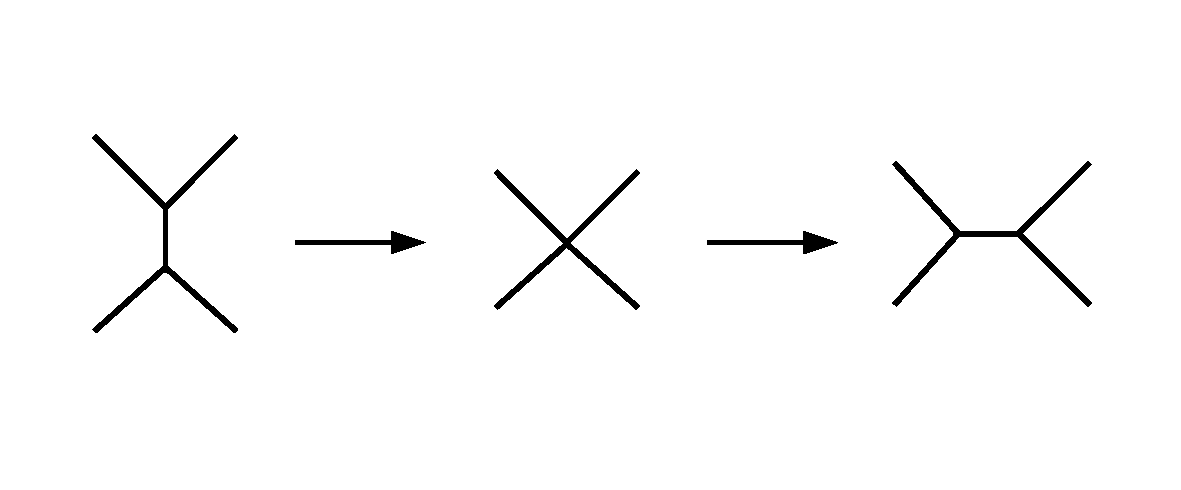
\includegraphics[scale=0.5]{flipping.pdf}
    \caption{Neighbor switching}
    \label{fig:flipping}
\end{figure}

\begin{figure}[t]
    \centering
    \includegraphics[scale=0.5]{removal.pdf}
    \caption{Grain removal}
    \label{fig:removal}
\end{figure}

\section{Topology of Grain Structures}

As stated before the grain structure is projected on a torus where each vertex is connected to three other vertices, and thus belongs to three boundaries. The structure has the following Euler characteristic considering the number of vertices $M$, the number of boundaries $K$ and the number of grains $N$ \cite{sausset2007periodic}:
\begin{equation}
M - K + N = 0
\label{eq:eulertorus}
\end{equation}
If we count the number of vertices in a grain structure we count three boundaries per vertex, but as each boundary is shared by two vertices, the boundaries are counted twice. Using these facts and considering \eqref{eq:eulertorus} we obtain the following relations:
\begin{align*}
    3\,M &= 2\,K\\
    N &= \frac{K}{3} = \frac{M}{2}
\end{align*}
 Consider an initial condition of a grain structure with $N_0$ number of grains, $M_0$ vertices and $K_0$ boundaries where $N_0 = M_0/2 = K_0 / 3$. 
 The topological transitions during grain structure evolution will change the number of these components. 
 The only topological transition considered that alter the number of components in a grain structure is  grain removal. 
 When a grain is removed, three boundaries and two vertices are removed, leaving a single \emph{survivor} vertex.
 Now assume that at a given time $t$ we started with $N_t$ grains and then we removed $n_t$ grains, leaving at the next time step $N_{t+1}$ grains.
 Topological transitions described induces that we removed exactly $3n_t$ boundaries and $2n_t$ vertices and the following definitions yields between vertices, boundaries and grains between time steps $t$ and $t+1$:
 \begin{align*}
     dN_t &= N_{t+1} - N_{t} =  - n_t\\
     dK_t &= K_{t+1} - K_{t} = - 3n_t\\
     dM_t &= M_{t+1} - M_{t} = - 2n_t.
 \end{align*}
We can build the following relation in terms of the variation of grains:
\begin{equation}
    3\,dM_t = 2\,dK_t. \label{eq:dMdK}
\end{equation}
If we add the variations over all the time steps, from time $t=0$ to $t=T$ we obtain:
\begin{align*}
    \sum_{t=0}^{T}3\,dM_t &= 3(M_1 - M_0 + M_2 - M_1 + \cdots + M_{T+1} - M_T) \\
    &= 3(M_{T+1} - M_0).
\end{align*}
\begin{align*}
    \sum_{t=0}^{T}2\,dK_t &= 2(K_1 - K_0 + K_2 - K_1 + \cdots + K_{T+1} - K_T) \\
    &= 2(K_{T+1} - K_0).
\end{align*}
This total variations for vertices and boundaries are equal according to \eqref{eq:dMdK}. By the fact that the initial condition is true, \ie  $3M_0 = 2K_0$, for a time $t=T$ the number of vertices and boundaries are related as:
\begin{align*}
    N_{T+1} &= \frac{M_{T+1}}{2}\\
    N_{T+1} &= \frac{K_{T+1}}{3}\\
    3M_{T+1} &= 2K_{T+1}.
\end{align*}
This implies that grain structure evolution holds the same relation between grains, boundaries and vertices along the simulation.
%%% Dynamics
\section{Curvature and Vertex Models}

The total energy of the grain structure depends on the individual energies along each grain boundary. The total energy thus takes the form:
\begin{equation}
    E(t) = \sum_{k=1}^{K} \int_0^1 \gamma ^{(k)}\norm{\mylvec^{(k)}(s,t)}\, ds,
    \label{eq:energy}
\end{equation}
where $\mylvec^{(k)}(s,t) = \dxids^{(k)}(s,t)$ is a tangent vector to $\vxi^{(k)}$ and $\norm{\cdot}$ is the $l^2$-norm. Grain system motion equations can be found from this equation by derivating it with respect to time. Computing the derivative of $\eqref{eq:energy}$ we obtain:
\begin{align}
    \dfrac{dE}{dt}(t) &= \sum_{k=1}^{K} \int_0^1 \gamma^{(k)} \unitlk \cdot \dlvecdt^{(k)}\!(s,t) \, ds \nonumber\\
    &= \sum_{k=1}^{K} \int_0^1 \gamma^{(k)}\, \T^{(k)}(s,t) \cdot \dvds^{(k)}\!(s,t) \, ds \label{eq:dEdt},
\end{align}
where $\T^{(k)}(s,t)$ is a unit tangent vector of the boundary and $\gamma^{(k)}\T^{(k)}$ it is called capillar force. Note that \eqref{eq:dEdt} is valid as long as $K'(t) = 0$ within $[t_1, t_2]$, \ie
there are not topological transitions. Integrating by parts \eqref{eq:dEdt} we obtain:
\begin{equation}
    \dfrac{dE}{dt}(t) = -\sum_{k=1}^K \int_0^1 \gamma^{(k)}\dTds^{(k)}\!\!\cdot \vel^{(k)}\, ds + \sum_{m=1}^M \vel_m \cdot \sum_{l=1}^{3} \gamma^{(m,l)}\T^{(m,l)}
    \label{eq:dEdtfull},
\end{equation}
In order to enforce the decreasing energy of the system we must ensure that \eqref{eq:dEdtfull} be negative. 
If we only consider the triple junction drag the boundaries becomes flat, therefore $\dTds^{(k)}\! = 0$ for each boundary. The triple junction velocity is set to decrease energy as:
\begin{equation*}
    \vel_{m} = - \lambda \gamma^{(m,l)}\T^{(m,l)},
\end{equation*}
where $\lambda$ is called triple junction mobility. This model is called Vertex model. On the other hand if we only consider the grain boundary influence, we can set the velocity to be proportional to the boundary normal vector, which yields the following expression for boundary velocity:
\begin{equation*}
    \vel^{(k)} = \mu \gamma^{(k)} \dTds^{(k)},
\end{equation*}
where $\mu$ is called boundary mobility. Since the motion is curvature-driven,\ie there is no triple junction influence, this model is called \emph{Curvature model}. A geometrical consequence under this model is the \emph{Herring condition} where the angle between boundaries, namely dihedral angle, is always $2\pi/3$ \cite{herring1951surface}. This comes from forcing the geometrical condition over tangent vectors:
\begin{equation}
    \sum_{l=1}^{3}\gamma^{(m,l)}\T^{(m,l)} = 0.
\end{equation}
Moreover the rate of growth for a grain becomes independent of its area, being proportional to the number of sides of the grain or grain class $\ns(g)$. This relation stablishes that a grain with $\ns(g) < 6$ will shrink and with $\ns(g) > 6$ will grow, in fact the case of 6-sided grain the rate of growth is zero. This relation is known as \emph{Von Neumann-Mullins relation} \cite{mullins1956two} and can be expressed as:
\begin{equation}
    \frac{dA}{dt}(g) = \frac{\nu}{3}(\ns(g)-6)
    \label{eq:vonneumann-mullins}
\end{equation}
where $\nu$ is a term proportional to grain boundary energies $\gamma^{(k)}$ and mobility $\mu$. Under constant $\gamma^{(k)}$, $\nu \propto \gamma \mu$.


%Thus we define the evolution equations for triple junctions and boundaries as:
%\begin{align}
    %\vel_m\,&= -\lambda \sum_{l=1}^3 \T^{(m,l)} \label{eq:vertexvelocity} \\
    %\vel^{(k)} &= \mu \dTds^{(k)}, \label{eq:boundaryvelocity} 
%\end{align}
%where $\lambda$ and $\mu$ are the mobilities for triple junctions and boundaries respectively. These mobility coefficients are introduced to separate the dynamics of the elements involved. When the mobility of the triple junction is higher than the mobility of the boundaries, triple junctions adjust quickly, this allows boundaries to obtain a curve shape. 

\chapter{Closed Boundary Motion}
\label{chap:closedboundary}

\lettrine{A}{n} interesting case of study for understanding mathematical and numerical aspects of grain growth simulation is to understand the evolution of a closed boundary which tries to minimize its energy. 
Let $\vxi(s,t) = \langle x(s,t), y(s,t)\rangle,\, s \in [0, 2\pi]$ a closed curve in $\Reals^2$ such that $\vxi(0,t) = \vxi(2\pi,t)$, where $s$ is the parametrization variable and $t$ is the time variable. 
This will be the base definition of a closed boundary. 
Let $\mylvec(s,t) = \dxids(s,t)$ a tangent vector to the boundary $\vxi$ and $\T(s,t) = \unitl$ the unit tangent vector in the same direction. 
Also let $\N(s,t) = \dTds(s,t)$ a unit normal vector to $\vxi$. 
From the total energy equation in \eqref{eq:energy}, the energy of this boundary becomes a single integral term:
\begin{equation}
    E(t) = \int_0^{2\pi} \norm{\mylvec(s,t)}\, ds,
    \label{eq:energyclosed}
\end{equation}
where for simplicity we assumed an isotropic regime, \ie $\gamma = 1$. 
Taking the derivative of \eqref{eq:energyclosed} with respect to the time yields:
\begin{equation}
    \dfrac{dE}{dt}(t) = \int_0^{2\pi} \unitl \cdot \dlvecdt(s,t) \, ds.
    \label{eq:dEdtclosed}
\end{equation}
Let $\vel(s,t) = \dxidt(s,t)$ the velocity of the boundary. Equation $\eqref{eq:dEdtclosed}$ becomes:
\begin{equation}
    \dfrac{dE}{dt}(t) = \int_0^{2\pi} \T(s,t) \cdot \dvds(s,t) \, ds.
    \label{eq:dEdtclosed2}
\end{equation}
Integrating by parts \eqref{eq:dEdtclosed2} we obtain:
\begin{align}
    \dfrac{dE}{dt}(t) &= \T(s,t)\cdot\vel(s,t)\eval{0}{2\pi} - \int_0^{2\pi}  \dTds(s,t) \cdot \vel(s,t) \, ds \nonumber\\
    &= -\int_0^{2\pi} \dTds(s,t) \cdot \vel(s,t)\, ds. \label{eq:dEdtclosed3}
\end{align}
Thus, we will use \eqref{eq:dEdtclosed3} to understand the motion of a closed boundary.

\section{Curvature based motion}

Curvature based grain growth models assumes that the velocity of the boundaries is in the direction of its normal vector and proportional to its curvature $\kappa(s,t)$~\cite{Kinderlehrer2006}. Thus the velocity of the boundary can be defined as~\cite{thomascalculus}:
\begin{equation}
    \vel(s,t) = \kappa(s,t)\N(s,t). %\label{eq:closedboundaryvelocity}
    \nonumber
\end{equation}
This term can be obtained also from the derivative of the vector $\T$ with respect to the arc length $\AL$:
\begin{align}
    \dTdAL(s,t)  &= \kappa(s,t)\N(s,t) \nonumber\\
    \dTds(s,t) \dsdAL &=\kappa(s,t)\N(s,t). \label{eq:dTdAL}
\end{align}
Let $\AL(s)$ the arc length of the boundary up to $s$, given by:
\begin{equation}
    \AL(s) = \int_0^{s} \norm{\mylvec(s,t)}\, ds,
    \label{eq:arclen}
\end{equation}
then we can obtain $\dsdAL$ from \eqref{eq:arclen} by derivating with respect to $s$ as:
\begin{align*}
    \frac{d\AL}{ds} &= \norm{\mylvec(s,t)} \\
    \frac{ds}{d\AL} &= \frac{1}{\norm{\mylvec(s,t)}}.
\end{align*}
Replacing in \eqref{eq:dTdAL} we obtain:
\begin{equation}
    \dfrac{1}{\norm{\mylvec(s,t)}} \dTds(s,t) = \kappa(s,t)\N(s,t).
    \label{eq:curvresult}
\end{equation}
Therefore to obtain curvature based motion we need to compute the grain boundary velocity as:
\begin{equation} \vel(s,t) = \frac{1}{\norm{\mylvec(s,t)}}\dTds(s,t). \label{eq:curvvelocity}
\end{equation}

\section{Motion for a Closed Boundary with Discrete Points}

%Let's consider the same boundary parametrization as the coupled model from \eqref{eq:boundarydiscret}. We do not need to handle a special treatment of vertices and interior points.
Let's consider the boundary $\vxi(s,t)$ and a continuous representation via the collocation points $\vertices = \{\x_1,\dotsc,\x_n\}$ and a interpolating function $\phi$ as:
\begin{equation}
    \vxi(s,t) = \boundarytwo,\quad s \in [0,2\pi].
\end{equation}
Due to our construction of the boundary, this interpolating function must preserve the periodicity. 
For example an interpolating function to be considered here is the periodic $\sinc$~\cite{trefethen2000spectral}. 
The velocity of the boundary $\vel$ is expressed in terms of the parametrization as:
%Since we are dealing with a periodic condition for this grain boundary, instead of classic Lagrange interpolating functions $\phi_i$, we should use another interpolation basis, for example the periodic sinc interpolator \cite{trefethen2000spectral}. The velocity of the boundary $\vel$ is expressed in terms of the parametrization as:
\begin{equation}
    \vel(s,t) = \velboundary.
\end{equation}
We can replace the velocity term in \eqref{eq:dEdtclosed3} to obtain the derivative of the energy in terms of the boundary.
\begin{align}
    \dfrac{dE}{dt}(t)
    &= -\int_0^{2\pi} \dTds(s,t) \cdot \left( \velboundary \right)\, ds \nonumber \\
    &= -\sum_{i=1}^{n}  \dotx[i](t) \cdot \int_0^{2\pi}  \dTds(s,t) \phii{i}{s}\, ds.
    \label{eq:dEdtboundclose}
\end{align}
The velocity at the boundary points $\x[i]$ can be defined from \eqref{eq:dEdtboundclose} such that decreases the energy of the grain system as:
\begin{equation}
    \dotx[i](t)= \frac{\zeta}{\norm{\mylvec(s_i,t)}}\int_0^{2\pi}  \dTds(s,t) \phii{i}{s}\, ds,
    \label{eq:coupledvelocity}
\end{equation}
%
where we introduced the curvature term from \eqref{eq:curvresult} for each discrete boundary point and a constant $\zeta$ which depends on the specific parametrization and interpolation and will be defined in the next section. 
This evolution equation differs with the curvature based evolution equation found before in \eqref{eq:curvvelocity}. 
Here we have instead a \emph{integral} normal vector at a given point along the boundary.
It can be seen as a smoothed normal term.
In order to %find more agreement with the curvature based 
understand this evolution equation, we will study a circular boundary in the next subsection, in which simple formulas can be obtained.

%The following sections shows the theoretical evolution of a circular boundary and how the discrete boundary equations successfully approaches the evolution. This result can be extended to general boundary shapes, whilst the theoretical ratios are not derived in the later, a generic boundary evolving and minimizing energy reaches a state where becomes a circle, and thus the prior results are again valid.

\subsection{Circular Boundary}
\label{sec:circularboundary}

This simple case is very illustrative, since we can obtain an explicit formula for $\dfrac{dE}{dt}$ and also the area rate of change $\dfrac{dA}{dt}$. 
First we describe analytic results for the boundary evolution and then we apply the coupled model idea to interpolate the boundary and obtain the new evolution equations.

The equation that describes this boundary is:
\begin{equation}
    \vxi(s,t) = R(t)\langle \cos(s), \sin(s) \rangle,\quad R(t) > 0 \;\;\forall\,t \geq 0,
    \label{eq:circle}
\end{equation}
where we have decoupled the spatial parametrization in polar coordinates with the radial time-dependence. Notice that $\norm{\vxi(s,t)} = R(t)$, that is, for a fixed time $t=\tau$, the boundary preserves a constant radius and thus constant curvature along the boundary. The tangent vector $\mylvec(s,t)$ is nothing but:
\begin{equation*}
    \mylvec(s,t) = R(t)\langle -\sin(s), \cos(s) \rangle,
\end{equation*}
and again its norm $\norm{\mylvec(s,t)} = R(t)$ just like $\vxi$. This implies that the unit tangent vector is:
\begin{equation*}
\T(s,t) = \langle -\sin(s), \cos(s) \rangle,
\end{equation*}
and the normal vector is:
\begin{equation*}
    \dTds(s,t) = \langle -\cos(s), -\sin(s) \rangle,
\end{equation*}
which is a vector always pointing to the circle center. If we took these results and plug them in \eqref{eq:dEdtclosed3} yields:
\begin{equation*}
    \dfrac{dE}{dt}(t) = \int_0^{2\pi}  \langle \cos(s), \sin(s) \rangle \cdot \vel(s,t)\, ds.
\end{equation*}
Considering that the boundary moves proportional to the curvature and in a normal direction, we replace the velocity term with the curvature result in \eqref{eq:curvresult}:
\begin{align}
    \dfrac{dE}{dt}(t) &= \int_0^{2\pi}  \langle \cos(s), \sin(s) \rangle \cdot \frac{1}{\norm{\mylvec(s,t)}} \langle -\cos(s), -\sin(s) \rangle\, ds \nonumber\\
    &= \int_0^{2\pi} -\frac{1}{R(t)} \,ds \nonumber\\
    &= -2\pi \kappa(t) \label{eq:dEdtcircle}
\end{align}

The rate of change of the area can also be obtained from the definition of area given the boundary parametrization in \eqref{eq:circle}:
\begin{align}
    A(t) &= \frac{1}{2} \int_0^{2\pi} \norm{\vxi(s,t)}^2\, ds\nonumber\\
    \dAdt(t) &= \int_0^{2\pi} \vxi(s,t)\cdot \vel(s,t)\,ds \nonumber\\
    &= \int_0^{2\pi} R(t)\langle \cos(s),\sin(s)\rangle \cdot \frac{1}{R(t)} \langle -\cos(s),-\sin(s)\rangle \,ds \nonumber\\
    &= -2\pi \label{eq:dAdtcircle}
\end{align}
This means that the rate of change for the area of a circle is constant. The evolution of the radius $R(t)$ over time can be explicitly found by comparing the velocity of the curvature in \eqref{eq:curvresult} with the circle velocity expression:
\begin{align}
    \frac{dR}{dt}(t) &= -\frac{1}{R(t)} \label{eq:circvel}\\
    %\frac{1}{2}(R(t)^2 - R(0)^2) &= t \\
    R(0) &= R_0, \nonumber
    %R(t) &= \sqrt{R_0^2 - 2t} \label{eq:radii},
\end{align}
where $R_0$ is the initial radius of the circle at time $t=0$. The solution therefore is,
\begin{equation}
    R(t) = \sqrt{R_0^2 - 2t}.
    \label{eq:radii}
\end{equation}
The solution is valid as long as $R_0^2 > 2t$. In the limit, the circle should become a single point, and the related vectors becomes indeterminate. Finally, the complete description of a circular boundary is given by:
\begin{equation}
    \vxi(s,t) = \sqrt{R_0^2 - 2t}\,\langle \cos(s), \sin(s) \rangle.
\end{equation}
The coupled model based formula induces a different result from the velocity found in \eqref{eq:circvel}. Assuming equispaced points in $[0, 2\pi]$, we replace $\mylvec$ and $\dTds$ for the circle in \eqref{eq:coupledvelocity} to obtain:
\begin{equation}
    \dotx[i](t) = \frac{1}{R(t)} \int_0^{2\pi}  \langle -\cos(s), -\sin(s)\rangle \,\phi_i(s)\, ds,
\end{equation}
where $\phi$ the periodic $\sinc$ interpolation function. Notice that this definition needs even number of discrete points. If we replace the definition of the periodic $\sinc$ we obtain:
\begin{align}
    \dotx[i](t) &= -\frac{1}{R(t)} \int_0^{2\pi} \left\langle \cos(s)\frac{\sin(\pi(s-s_i) / h)}{\frac{2\pi}{h} \tan((s-s_i)/2)}, \sin(s)\frac{\sin(\pi(s-s_i) / h)}{\frac{2\pi}{h} \tan((s-s_i)/2)} \right\rangle\,ds\\
    &= -\frac{1}{R(t)}  \frac{2\pi}{n}\left\langle\cos \left(\frac{2\pi i}{n}\right), \sin\left(\frac{2\pi i }{n}\right)\right\rangle.
    \label{eq:curvaturevelocity}
\end{align}
Under the $\sinc$ interpolant, the constant $\zeta$ from \eqref{eq:coupledvelocity} becomes $2\pi/n$. Figure \ref{fig:circularboundary} shows the evolution of the boundary with 14 points using the velocity equation from \eqref{eq:curvaturevelocity}. The discrete data is extracted from a circle and then is interpolated using the sinc periodic interpolator. For this example we set $R_0 = 2$, which implies that the limit time of the simulation is $t_{\text{lim}}=2$. The theoretical description of the circle matches qualitatively with the interpolated curve, and for simplicity of presentation the theoretical circle is not shown. 

\begin{figure}[t]
    \centering
    \includegraphics[scale=0.6]{closed_boundary/circularboundary.pdf}
    \caption[Circular boundary evolution]{Evolution of circular boundary. Velocity vectors are marked in blue gradient, white for the smallest vector and blue for the largest. (Top left) The initial condition at $t=0$ of the circular boundary with $R_0 = 2$. (Top right, bottom left) After some time the circle start to shrink and the velocity of the boundary increases. (Bottom right) Near $t=2$ the circle becomes smaller and the velocity vectors increased their magnitude.}
    \label{fig:circularboundary}
\end{figure}

Figures~\ref{fig:circularboundary_area} and ~\ref{fig:circularboundary_energy} shows relevant statistics of the experiment. Boundary area is in good agreement with the theoretical area. Area rate of change shows that whilst we should expect exactly $\dAdt = -2\pi$, we get some oscillations around this value, increasing in magnitude as simulation reaches $t_{\text{lim}}$. Actually the simulation is stopped at some time before reach $t_{\text{lim}}$, because of the mentioned acceleration of the circular boundary. The grain boundary energy under isotropic regime becomes just the perimeter of the circle $P(t) = 2\pi R(t)$. The measured energy of the simulated circle is a monotonic decreasing function in good agreement with the theoretical perimeter obtained from the radii in \eqref{eq:radii}, as well as the rate of change of the energy. 

\begin{figure}[t]
    \centering
    \includegraphics[scale=0.55]{closed_boundary/circularboundary_area.pdf}
    \subfloat[\label{fig:area}]{\hspace{.55\linewidth}}
    \subfloat[\label{fig:dAdt}]{\hspace{.45\linewidth}}
    \caption[Circular boundary area and rate of change]{(a) Circle area is in good agreement with the theoretical description. (b) Rate of change is not constant in the numerical simulation, but it is near the theoretical value.}
    \label{fig:circularboundary_area}
\end{figure}

\begin{figure}[t]
    \centering
    \includegraphics[scale=0.55]{closed_boundary/circularboundary_energy.pdf}
    \subfloat[\label{fig:circenergy}]{\hspace{.55\linewidth}}
    \subfloat[\label{fig:circdEdt}]{\hspace{.45\linewidth}}
    \caption[Circular boundary energy and rate of change]{(a) Grain energy function is in good agreement with the evolution of the perimeter of the circle. (b) Rate of change of the energy, in agreement with the precipitation of the boundary motion as the radio goes to zero.}
    \label{fig:circularboundary_energy}
\end{figure}

\subsection{Non-regular Boundary}

Most grains and their boundaries are not restricted to hold circular shapes. The following example shows a boundary described by a polar rose with an initial condition:
\begin{equation*}
    \vxi(s,0) = 3 + \cos(3s)
\end{equation*}
using 14 interpolation points. The number of points is chosen merely to resemble the interpolated function. The simulation is performed using the curvature equations from \eqref{eq:curvaturevelocity}. 

Figure~\ref{fig:nonregularboundary} shows the evolution of the polar rose. The equations used ensures energy minimization, which induces that the velocity of the discrete points lying in the concave sections points outside the the rose, trying to achieve some iterations later a fully convex form. In the convex form now the points try to approximate a circle shape, which leads to the known evolution presented in Section~\ref{sec:circularboundary}. Figures~ \ref{fig:nonregularboundary_area} and~ \ref{fig:nonregularboundary_energy} shows relevant statistics of the experiment. The polar rose area shows qualitatively linear behavior, but a closer look to the derivative shows that there is some perturbation during the minimization, which is soften towards the end of the simulation. The grain boundary energy shows a monotonic decreasing behavior, and its derivative shows a transient where the derivative becomes less negative due to the polar rose correcting its concave parts. After the rose becomes a convex figure, the derivative becomes more and more negative, until numerical collapse at the end of the evolution.

\begin{figure}[t]
    \centering
    \includegraphics[scale=0.6]{closed_boundary/nonregularboundary.pdf}
    \caption[Non-regular boundary evolution]{Evolution of non-regular boundary. Velocity vectors are marked in blue gradient, white for the smallest vector and blue for the largest.
    (Top left) The initial condition at $t=0$ for the polar rose. (Top right) After some time the boundary is driven to correct the curvature while trying to minimize energy. (Bottom left) The boundary is completely convex and all the velocity vectors points to the interior. (Bottom right) The polar rose now has a circle-like shape and the velocity vectors tends to point to the center.}
    \label{fig:nonregularboundary}
\end{figure}



\begin{figure}[t]
    \centering
    \includegraphics[scale=0.55]{closed_boundary/nonregularboundary_area.pdf}
    \subfloat[\label{fig:noncircarea}]{\hspace{.55\linewidth}}
    \subfloat[\label{fig:noncircdAdt}]{\hspace{.45\linewidth}}
    \caption[Non-regular boundary area and rate of change]{(a) Polar rose area shows qualitatively linear behavior, as expected. (b) Rate of change is not constant in the numerical simulation but tries to stabilize.}
    \label{fig:nonregularboundary_area}
\end{figure}

\begin{figure}[t]
    \centering
    \includegraphics[scale=0.55]{closed_boundary/nonregularboundary_energy.pdf}
    \subfloat[\label{fig:noncircenergy}]{\hspace{.55\linewidth}}
    \subfloat[\label{fig:noncircdEdt}]{\hspace{.45\linewidth}}
    \caption[Non-regular boundary energy and rate of change]{(a) Grain energy function shows a monotonic decreasing behavior. (b) Rate of change of the energy collapses at the end of the simulation, meaning that the polar rose is becoming a single point.}
    \label{fig:nonregularboundary_energy}
\end{figure}

\chapter{The Coupled Model}
\label{chap:coupledmodel}

\lettrine{N}{umerical} simulations studied by vertex-driven motion and curvature-driven motion as exposed in Chapter \ref{chap:2dgrains} can be also studied in a coupled way with the purpose of capturing the dynamics of both models and being able to reproduce each one of them individually. This novel model is called Coupled Model and has been developed in a first version in \cite{bachelorthesisasazo} and improved during the study of the present work. The boundary parametrization proposed here consist in a Lagrange interpolation of $n$ points as follows:
\begin{equation}
    \vxi(s,t) = \boundary,\quad s \in [0,1],
    \label{eq:boundarydiscret}
\end{equation}
where $\phi_i(s)$ are the Lagrange interpolation functions and the points $\x[1]^{(k)}$ and $\x[n]^{(k)}$ are triple junctions. The remaining $n-2$ collocation points are called interior points. For numerical stability each point $\x[i]^{(k)}$ is parametrized on Chebyshev nodes of the second kind\cite{trefethen2000spectral} with a linear transformation to stay in the domain $[0,1]$.

We start with the derivative of the total energy of the grain structure in \eqref{eq:dEdtfull} and we replace the proposed parametrization as:
\begin{equation}
    \frac{dE}{dt}(t) = \int_0^1 -\sum_{k=1}^{K}\left[ \sum_{i=1}^{n} \dotx[i][k](t)  \cdot \int_0^1  \gamma^{(k)}\dTds^{(k)}\!\! \phi_i(s)\,ds \right] + \sum_{m=1}^{M} \vel_m(t) \cdot \sum_{l=1}^3 \gamma^{(m,l)}\T^{(m,l)}.
    \label{eq:dEdtcoupled1}
\end{equation}
In order to find the motion equations of the system we separate the terms related to triple junctions from the summatory over grain boundaries in \eqref{eq:dEdtcoupled1} as:
\begin{multline*}
    \frac{dE}{dt}(t) =  -\sum_{k=1}^{K}\left[ \sum_{i=2}^{n-1} \dotx[i][k](t)  \cdot \int_0^1  \gamma^{(k)}\dTds^{(k)}\!\! \phi_i(s)\,ds \right] + \sum_{m=1}^{M} \vel_m(t) \cdot \sum_{l=1}^3 \gamma^{(m,l)}\T^{(m,l)} + \\ \sum_{k=1}^K \left[\dotx[1][k](t)\cdot\int_0^1 \gamma^{(k)} \dTds^{(k)}\!\! \phi_1(s)\,ds + \dotx[n][k](t)\cdot\int_0^1 \gamma^{(k)} \dTds^{(k)}\!\! \phi_n(s)\,ds\right].
\end{multline*}
Then we add them up to the former triple junction term. Notice that we must choose which contribution (from $\x[1][k]$ or $\x[n][k]$) will be added, since for some arbitrary pair of boundaries $k_1, k_2$, $\x[1][k_1] = \x[n][k_2]$ and we would be adding repeated terms. Re-indexing this contribution in terms of the triple junctions we obtain:
\begin{multline}
    \frac{dE}{dt}(t) =   -\sum_{k=1}^{K}\left[ \sum_{i=2}^{n-1} \dotx[i][k](t)  \cdot \int_0^1  \gamma^{(k)}\dTds^{(k)}\!\! \phi_i(s)\,ds \right] + \sum_{m=1}^{M} \vel_m(t) \cdot \sum_{l=1}^3 \gamma^{(m,l)}\T^{(m,l)} - \\ \sum_{m=1}^{M} \dotx[m]\,\,(t) \cdot \sum_{l=1}^3 \int_0^1 \gamma^{(m,l)} \dTds^{(m,l)}\phi_{1,m}(s)\,ds.
    \label{eq:dEdtcoupled3}
\end{multline}
where $\vel_m = \dotx[m]$. From Chapter \ref{chap:closedboundary}, we can obtain curvature driven motion if we add in the curvature term $1/\norm{\mylvec(s,t)}$ from \eqref{eq:coupledvelocity} to the velocity of the interior points. Thus, the motion equations of the improved model are:
\begin{align}
    \dotx[i][k](t) &= \frac{\mu\gamma^{(k)}}{\norm{\mylvec(s_i,t)}} \int_0^1 \dTds^{(k)}\!\!\phi_i(s)\,ds \\
    \dotx[m]\,\,(t) &= -\lambda\sum_{l=1}^{3}\gamma^{(m,l)} \left[\T^{(m,l)} - \int_0^1 \dTds^{(m,l)}\,\phi_{1,m}(s)\,ds \right],
\end{align}
where $\lambda$ and $\mu$ are the mobilities for interior points, inherited from boundary motion, and lambda is the triple junction mobility.
\section{Numerical Implementation}

An important result of the study of extinction time is that topological transitions are delayed because the extinction time estimation has an error proportional to the simulation $\Delta t$. This study suggest that the continuous motion of triple junctions and boundaries must be accurate enough to estimate extinction times of higher order. 

The first idea to obtain a better approximation of extinction time is to perform $r$ steps of size $\Delta \tau$ such that $\Delta \tau = \Delta t / r$. During the execution of this steps, the basic assumption is that no topological transition occurs and thus the system just evolves. Using a smaller time step helps to ensure a better approximation. On the other hand, straightforward higher order methods can be used. For example second order Runge-Kutta ensures that the grain system evolves with precision $\mathcal{O}(\Delta t^2)$, and therefore the extinction time has the same precision. Runge-Kutta can also be improved by the introduction of many steps of smaller size. 
In both methods, topological transitions that might occur in $[t, t+\Delta t]$ are detected and managed after the evolution is performed. Both methods are discussed below.

\subsection{Multistep Euler}

This method assumes that Euler method can be improved if steps of smaller size are performed to evolve the grain structure previous to handle topological transitions. A number $r$ of smaller steps of size $\Delta \tau$ is chosen, where $\Delta \tau = \Delta t / r$. The execution of this $r$ steps is called the \emph{multistep stage} and the system evolves assuming that there are not topological transitions. Algorithm \ref{alg:multistep} shows this method.

\begin{algorithm}
\caption{Multistep Euler for Coupled Model}
\label{alg:multistep}
\begin{algorithmic}[1]
\Procedure{ME}{}
\State $\Delta \tau \gets \dfrac{\Delta t}{r}$ Time step of multistep phase.
\For{$k:1,\dotso,r$}
%\State Detect Topological Transitions
\State $\mathbf{V}_t \gets$ Compute velocities
\State $X_{t + \Delta \tau} \gets X_{t} + \Delta \tau \mathbf{V}_t$
\State $t \gets t + \Delta \tau$
\EndFor
\EndProcedure
\end{algorithmic}
\end{algorithm}

Using a smaller step-size helps to ensure a better approximation of the extinction time proportional to $\mathcal{O}(\Delta \tau)$.
Inside the multistep stage, topological transitions are detected by computing the extinction time of the boundaries and comparing it with $\Delta t$ but they are not performed. When the multistep stage is over all the topological transitions found are filtered so there are no inconsistencies and then are performed safely. No extra memory is required for this method, but the cost if purely computational since the method is performing $r$ steps per main step and thus is almost $r$ times slower.  Notice that when $r = 1$, we recover the original Forward Euler method.

\subsection{Multistep Second Order Runge-Kutta}

If the goal is to obtain a good approximation of the extinction time, a higher order method can be implemented straightforward. For example extinction times with precision $\mathcal{O}(\Delta t^2)$ can be estimated using second order Runge-Kutta (RK2). We can also improve this method by means of introducing the multistep idea to perform several RK2 steps within $[t,t+\Delta t]$ as shown in Algorithm \ref{alg:rk2}.

\begin{algorithm}
\caption{Multistep Second Order Runge-Kutta for Coupled Model}
\label{alg:rk2}
\begin{algorithmic}[1]
\Procedure{MRK2}{}
\State $\Delta \tau \gets \dfrac{\Delta t}{r}$ Time step of multistep phase.
\For{$k:1,\dotso,r$}
\State $\mathbf{\overline{X}}_t \gets$ Backup positions $\mathbf{X}_t$ of triple junctions and interior points
\State $\mathbf{V}_t \gets$ Compute velocities
\State $\mathbf{X}_{t + \Delta \tau / 2} \gets \mathbf{X}_t + \dfrac{\Delta \tau}{2} \mathbf{V}_t$. Evolve structure for first RK estimation
\State $\mathbf{V}_{t + \Delta \tau /2} \gets$ Compute velocities
\State $\mathbf{X}_{t + \Delta \tau} \gets \mathbf{\overline{X}}_t + \Delta \tau \mathbf{V}_{t + \Delta \tau /2}$ . Evolve structure for second RK estimation
\State $t \gets t + \Delta \tau$
\EndFor
\EndProcedure
\end{algorithmic}
\end{algorithm}

The cost of this method lies in the memory needed to store the extra data for performing the two estimations at time $\Delta \tau/2$ and $\Delta \tau$ and the number of steps $r$. Notice that when $r = 1$  we recover the original RK2. In this implementation it is only necessary to backup the positions of the vertices and interior points to be used in the last step of the method and not the whole data structure \ie arc lengths, curvatures, grain areas, etc.

\subsection{Convergence Analysis of Extinction Time Estimation}
\chapter{The Continuous Stored Energy Vertex Model}
%\section{The Continuous Stored Energy Vertex Model}
\label{chap:storedenergy}

\section{Introduction}

\emph{Comment: The Introduction is for now a copy and paste
of what we had in dropbox paper. It will be improved asap.}


\begin{itemize}
    \item 
\textbf{NUCLEATION GROWTH PROCESSES: A MONTE CARLO SIMULATION (1977)}

Nucleation in layers.

\item \textbf{On Abnormal Subgrain growth and the origin of recrystallization nuclei (2003)}

\url{https://www.sciencedirect.com/science/article/pii/S135964540300079X}
Abnormal (The preferential or discontinuous evolution of a few grains in a polycrystal is termed abnormal grain growth) subgrain growth (grain inside grain) was found to be a plausible nucleation mechanism for recrystallization. They are not seeded in any form, emerges spontaneously. MC method used for simulation and comparison with experimental data.

\item \textbf{Recrystallization study using two-dimensional vertex model (2005)}

\url{https://yadda.icm.edu.pl/baztech/element/bwmeta1.element.baztech-article-BSW3-0014-0007}

Initial configuration: topology, orientations and stored energy. They aim to predict texture and microstructure modification during recrystallization. Inputs for the model are deformation texture, stored energy distribution and initial microstructure obtained from experiments.
Here the stored energy is introduced because allows nucleation. New nuclei are placed at the beginning of simulation with initial stored energy zero. Two nucleation were tested: random and proportional to the stored energy of the previous grain. Prefered nucleation predicts more correct texture change. Stored energy relative units range from 3 to 6.

\item \textbf{Generalized vertex model of recrystallization - Application to -polycrystalline copper (2008)}

\url{https://www.sciencedirect.com/science/article/pii/S0927025607002819}
“It is well known that recrystallization can significantly modify the distribution of orientations (texture) inside the material and produce drastic changes of many physical properties (electrical resis- tance, internal stresses, micro-hardness, etc.)”. Stored energy values are experimentaly obtained via x rays. Comparison of SE distribution, Boundary Misorientation distribution and texture (orientation).
Disadvantages for us: Uses SE with a vertex model.
Advantages for us: They don’t analyze mathematically when a nucleation will be successful ($\Delta$ SE). They mention (at the end) that they can’t compute MDF and ODF since they have few grains. There isn’t any computational implementation discussion.

\item \textbf{On the widths of orientation gradient zones adjacent to grain boundaries (2009)}

\url{https://www.sciencedirect.com/science/article/pii/S1359646209002589}
Paper aboux experimental results of orientations in grains. Does not mention recrystallization process (they do work over recrystallized material), stored energy nor nucleation.

\item \textbf{Level set framework for the finite-element modelling of recrystallization and grain growth in polycrystalline materials (2010)}

\url{https://www.sciencedirect.com/science/article/pii/S1359646210007906}
Model implemented a set of convection-reinitialization-diffusion equations with finite elements. Nucleation is implemented by introducing new grains based on some probabilistic or deterministic criteria. The sites for nucleation can be chosen randomly, at grain boundaries or according to criteria based on previous deformation step of polycrystal. Implementation in Cimlib C++ library. Three examples to show the capabilities of the model are presented. First is the motion of a vertex given a grain with a certain stored energy and its steady state and the motion of a vertex with an unstable initial condition and uniform SE in grains that reaches a steady state also. Second, an example with 1000 grains of isotropic grain growth and Third, 100 initial grains with random stored energy distribution and 200 new grains for nucleation with SE= 0, snapshots of different process (primary recrystallization and grain growth) are shown.

\item \textbf{Monte Carlo model in metal recrystallization simulation (2011)}

\url{https://link.springer.com/article/10.1007/s12204-011-1156-x}
Again an improved MC model which aims to simulate non-homogeneous recrystallization, the model does not take in account texture, thus results on isometric grains and experimental isometric grains differ because the model does not take in account the preffered growth orientation. Simulated grain size is less than experimental results.

\item \textbf{Interplay of kinetics and microstructure in the recrystallization of pure copper: Comparing mesoscopic simulations and experiments (2012)}

\url{https://link.springer.com/article/10.1007/s11661-012-1094-8}
The simulated microstructures after recrystallization exhibit a bimodal grain-size distribution instead of the broad, monomodal grain-size distribution found in the experiments. Cellular automaton model. Something about nucleation nature “‘Nucleation’’ in recrystallization is not a fluctuation phenomenon like in (solid–solid) phase transformations. Instead, the ‘‘nuclei’’ are present already in the deformed material in the form of subgrains that can become ‘‘activated’’ or ‘‘supercritical,’’ i.e., become ‘‘nuclei,’’ if certain instability criteria are (all) fulfilled”
“double-logarithmic plot of the recrystallized fraction as function of time”

\item \textbf{Investigation of nucleation and grain growth in 2-dimensional systems by using generalized Monte Carlo simulations (2013)}

\url{https://www.sciencedirect.com/science/article/pii/S0378437113003531}

2D generalized montecarlo simulation, achieves better result locating energy minima

\item \textbf{An Extended Vertex and Crystal Plasticity Framework for Efficient Multiscale Modeling of Polycristalline Materials (2017)}

\url{https://www.sciencedirect.com/science/article/pii/S0020768317303268#bib0031}
This multiscale modeling couples extended vertex model and crystal plasticity formulation. Allows stored energy, nucleation, pinning. GPU-implementation of the crystal plasticity component. They mention that there is no model where crystal plasticity is coupled to vertex model formulation. They also mention some vertex models that only consider grain growth and do not include influence or stored energy and anisotropic grain boundary properties. They mention that Piekos does not consider pinning nor anisotropic GB properties. Topological transitions are based on minimum length  $\Delta$ (so, this could also be studied). With introduction of SE they implement topological transition to break a grain (see Piekos 2005). Nucleation is placed in TJ and along grain boundaries. They do not mention numerical limits for SE effects. Tested on copper data.
Disadvantage for us: They study a similar model and work with Physical parameters. 
Advantages for us: It is still an active research topic, they only added a GPU-implementation for a small part of the model. The code is not available. They don’t study mathematica properties of the model (effect of SE to TJ, $\Delta$ SE min for nucleation).
\end{itemize}

\subsection{Overall Review}

It seems that nucleation mechanisms and simulations are compared with textures like copper and heavily deformed structures.
Orientation distribution function and misorientation distribution are studied from experimental data.  This experimental data also is used as input for configuration in simulations in, e.g. the varied MC models.
We also found coupled variation to obtain simulation for nucleation, primary recrystallization and grain growth. This kind of models (adaptation of vertex model) required certain topological transition to be stable.
The two most important “newer” papers are:
1.- Generalized vertex model of recrystallization - Application to -polycrystalline copper (2008)
2.-An Extended Vertex and Crystal Plasticity Framework for Efficient Multiscale Modeling of Polycristalline Materials (2017)

Another important paper is: Level set framework for the finite-element modelling of recrystallization and grain growth in polycrystalline materials, because they numerically study the role of SE for a vertex but they do their mathematical analysis. This is what we did with @Alejandro S for the poster we presented. So, it is worth to explain in detail.

\section{Related work}

 \lettrine{E}{xtension} of the classic vertex model considers the introduction of an intragranular stored energy $\SE$ which plays a key role in primary recrystallization. This process can significantly modify the distribution of orientations inside the material and produce drastic changes of many physical properties like electrical resistance, internal stresses, micro-hardness, etc.\cite{pikekos2008generalized, pikekos2008stochastic}
 The local energy of a vertex $i$ considering the stored energy term can be defined as:
 \begin{equation}
     E_i(t) = \sum_{j \in \mathcal{N}_i}\left(\gamma_{i,j}\AL_{i,j}(t) + \SE_{i,j}A_{i,j}(t)\right),
 \end{equation}
 %
 where $\mathcal{N}_i$ is the set of neighbor vertices to the vertex $i$, $\AL_{i,j}$ is the arc length of the boundary formed by vertices $i$ and $j$, $\SE_{i,j}$ and $A_{i,j}$ is the stored energy and area of a grain adjacent to the boundary $i,j$ using the right-hand rule. We split the local energy between the grain boundary contribution and the grain area contribution, so:
 \begin{equation}
     E_i(t) = \sum_{j \in \mathcal{N}_i}\gamma_{i,j}\AL_{i,j}(t) + \sum_{g \in \mathcal{G}_i} \SE_{g}A_{g}(t),
 \end{equation}
 %
 where $\mathcal{G}_i$ is the set of grains associated to vertex $i$. Now, we could define the total energy of the system as:
 \begin{equation}
     E(t) = \sum_{k \in \boundaries}\gamma_{k}\AL_{k}(t) + 
     \sum_{g \in \mathcal{G}} \SE_{g}A_{g}(t),
     \label{eq:SEtotalenergy}
 \end{equation}
 %
 where $\boundaries$ is the set of all the boundaries in the grain structure
 and $\mathcal{G}=\bigcup_i \mathcal{G}_i$ is the set of grains.
 So, now we could decompose the contribution
 from each vertex to the total energy as follows,
 %
 \begin{equation}
     \widehat{E}_i(t) = \sum_{j \in \mathcal{N}_i}\gamma_{i,j}\dfrac{\AL_{i,j}(t)}{2} + \sum_{g \in \mathcal{G}_i} \SE_{g}\dfrac{A_{g}(t)}{\ns(g)},
         \label{eq:SEvertexenergy}
 \end{equation}
 %
 where $\ns(g)$ is the number of sides (or class) of grain $g$. 
 This allows us to build the total energy
 as the sum of the contribution of each vertex
 such that we ensure we only consider once
 each grain boundary contribution and also consider
 once each grain contribution, thus,
 %
\begin{align*}
     \sum_{i \in \mathcal{N}}\widehat{E}_i(t) &=
     \sum_{i \in \mathcal{N}}\left(
     \sum_{j \in \mathcal{N}_i}\gamma_{i,j}\dfrac{\AL_{i,j}(t)}{2} + \sum_{g \in \mathcal{G}_i} \SE_{g}\dfrac{A_{g}(t)}{\ns(g)}\right) \\
     &=
     \underbrace{\sum_{i \in \mathcal{N}}\left(
     \sum_{j \in \mathcal{N}_i}\gamma_{i,j}\dfrac{\AL_{i,j}(t)}{2}\right)}_{(a)}  + 
     \underbrace{\sum_{i \in \mathcal{N}}\left(\sum_{g \in \mathcal{G}_i} \SE_{g}\dfrac{A_{g}(t)}{\ns(g)}\right)}_{(b)}
 \end{align*}
In order to solve $(a)$ we need to understand which elements are being counted. The outer sum takes all the vertices and the inner sum takes the neighbor vertices of each vertex. Consider the expanded terms for some vertex $k$:
\begin{equation*} \gamma_{k,j_1} \frac{\AL_{k,j_1}(t)}{2} + 
\gamma_{k,j_2} \frac{\AL_{k,j_2}(t)}{2} +
\gamma_{k,j_3} \frac{\AL_{k,j_3}(t)}{2},
\end{equation*}
where $j_1, j_2, j_3$ are the three neighbor vertices of vertex $k$. Let's see now the terms associated to one of these vertices, for example $j_1$:
\begin{equation*} \gamma_{j_1,k} \frac{\AL_{j_1,k}(t)}{2} + 
\gamma_{j_1,j_{12}} \frac{\AL_{j_1,j_{12}}(t)}{2} +
\gamma_{j_1,j_{13}} \frac{\AL_{j_1,j_{13}}(t)}{2}.
\end{equation*}
It is clear that for each vertex we are counting the energy associated to each boundary twice, each per vertex in a boundary. This justifies the introduction of the term $1/2$ in $\widehat{E}_i(t)$. The analysis to solve $(b)$ is similar. The inner sum of here runs over the grains related to vertex $i$. We can build a similar example starting from a vertex $k$ and counting the three stored energy terms related as:
\begin{equation*}
    \SE_{g_1} \frac{A_{g_1}(t)}{\ns(g_1)}+
    \SE_{g_2} \frac{A_{g_2}(t)}{\ns(g_2)}+
    \SE_{g_3} \frac{A_{g_3}(t)}{\ns(g_3)}
\end{equation*}
Consider now that $g_1$ has $\ns(g_1)$ vertices. We already know that $k$ is a vertex of $g_1$, the terms related to the $\ns(g_1) -1 $ remaining vertices must have a term $\SE_{g_1} \dfrac{A_{g_1}(t)}{\ns(g_1)}$ and thus we are summing in $(b)$ the same term $\ns(g_1)$ times. Of course, for any grain $g$ the times the related stored energy term is being added $\ns(g)$ times. This justifies the introduction of the term $1/\ns(g)$. Finally we can map the sum in order to count boundaries and grains. Each term related to a boundary is counted twice and each term related to a grain is counted $\ns(g)$ times and we can recover an expression for the total energy of the system as:

 \begin{align*}
     \sum_{i \in \mathcal{N}}\widehat{E}_i(t) &= \sum_{k \in \boundaries}2\,\gamma_{k}\dfrac{\AL_{k}(t)}{2} + 
     \sum_{g \in \mathcal{G}} \ns(g)\,\SE_{g}\dfrac{A_{g}(t)}{\ns(g)}\\
      &= \sum_{k \in \boundaries}\gamma_{k}\AL_{k}(t) + 
     \sum_{g \in \mathcal{G}} \SE_{g}A_{g}(t) \nonumber\\
     &=E(t).
 \end{align*}
 %
 %
Notice that $\widehat{E}_i(t)$ is different
from $E_i(t)$.
%If we had just added up $E_i(t)$ to build
%the total energy, we would have counted
%each grain boundary contribution twice
%and each grain contribution proportional
%to the number of sides of each grain.

The boundary arc length $\AL$ and grain area $A$ can be seen as function of the vertices positions $\{\x_i\}$. Rewriting \eqref{eq:SEvertexenergy} marking this dependence as:
\begin{equation}
    \widehat{E}_i(\x(t)) = \sum_{j \in \mathcal{N}_i}\gamma_{i,j}\dfrac{\AL_{i,j}(\x)}{2} + \sum_{g \in \mathcal{G}_i} \SE_{g}\dfrac{A_{g}(\x)}{\ns(g)},\label{eq:vertexenergy}
\end{equation}
The evolution of the system, considering the stored energy term, such that it decreases energy
is obtain by a gradient descent method, so
$\dotx_i(t) = -\dfrac{\partial E}{\partial \x_i}$ for each vertex.

\section{Implementation}
Computing the velocity of each vertex is actually the computation of the gradient $\nabla_{\x}E$. 
Here we propose a matrix-free approach to approximate the gradient.
The main advantage of this approach is that it only needs the implementation of computation of the energy of the system, this simplifies enormously the bookkeeping we would need to handle this task.

A convenient approximation to compute $\dfrac{\partial E(\X)}{\partial \x_i}$ is to perform a matrix-free approach. 
Consider the vector $\X \in \mathbb{R}^{2n}$ of stacked components of $\x_i =(x_i, y_i)$, this is $\X = (x_1, x_2, \cdots, x_n, y_1, y_2, \cdots, y_n)^T$ where $n$ is the total number of triple junctions. 
Each $k$-th component of the gradient for this vector, say $\dfrac{\partial E(\X)}{\partial \X_k}$ is approximated by:
\begin{equation}
    \frac{\partial E(\X)}{\partial \X_k} \approx 
    \frac{E(\X + \varepsilon\,  \ei{k}) - E(\X)}{\varepsilon},
    \label{eq:partialE}
\end{equation}
where $\ei{k}$ is the $k$-th canonical vector in $\mathbb{R}^{2n}$. 
The numerical evaluation of this approximation implies that the energy of the system must be recomputed twice for each vertex, and according to \eqref{eq:SEtotalenergy} this means to recompute each individual vertex energy each time.
Fortunately, 
%this can improved.
this can be handled efficiently by pointing out which terms will change after the perturbation.

This quadratic cost required for a naive implementation is not real in practice. 
%as we explain here. 
A more detailed analysis shows that the perturbation only affects the $x$ or $y$ component of a vertex $\x_i$, which implies that only the three related grain areas and the three grain boundary arc-lengths will change as shown in Figure \ref{fig:delta_energy}.
%Thus the total energy changes only for the vertex $i$ and its three neighbors as shown in Figure \ref{fig:delta_energy}.
Thus the total energy is modified by each vertex that has a perturbed arc-length or area, that is, for each vertex belonging to the grains of $\x_i$.

\begin{figure}[t]
    \centering
    \begin{tikzpicture}
        % boundaries
        % grain 1
        \draw[line width=0.3mm, black] (0,0) -- (3,0.6);
        \draw[line width=0.3mm, black] (3,0.6) -- (3.6,-0.5);
        \draw[line width=0.3mm, black] (3.6,-0.5) -- (2.5, -3);
        \draw[line width=0.3mm, black] (2.5,-3) -- (0.1, -2.5);
        \draw[line width=0.3mm, black] (0.1,-2.5) -- (0,0);
        % grain 2
        \draw[line width=0.3mm, black] (2.5,-3) -- (0.1, -2.5);
        \draw[line width=0.3mm, black] (0,0) -- (-2, 1);
        \draw[line width=0.3mm, black] (-2,1) -- (-4, -1);
        \draw[line width=0.3mm, black] (-4,-1) -- (-2.5, -4);
        \draw[line width=0.3mm, black] (-2.5,-4) -- (0.1, -2.5);
        % grain 3
        \draw[line width=0.3mm, black] (-2,1) -- (-2.5, 2.5);
        \draw[line width=0.3mm, black] (-2.5,2.5) -- (-1.1, 3.5);
        \draw[line width=0.3mm, black] (-1.1,3.5) -- (1,3);
        \draw[line width=0.3mm, black] (1,3) -- (3,2);
        \draw[line width=0.3mm, black] (3,2) -- (3,0.6);
        % Perturbed data
        \draw[line width=0.3mm, red] (0.3,0) -- (3,0.6);
        \draw[line width=0.3mm, red] (0.3,0) -- (-2,1);
        \draw[line width=0.3mm, red] (0.3,0) -- (0.1,-2.5);
        % vertices
        \filldraw [black] (0,0) circle (1.2pt);
        \filldraw [black] (3,0.6) circle (1.2pt);
        \filldraw [black] (-2,1) circle (1.2pt);
        \filldraw [black] (0.1,-2.5) circle (1.2pt);
        \filldraw [red] (0.3,0) circle (1.2pt);
        \node[draw=none, color=black] at (-0.3, -0.2) {$\x_i$};
        \node[draw=none, color=red] at (1.5, -0.2) {$\x_i + \langle \varepsilon,0 \rangle$};
        \node[draw=none, color=black] at (3.5, 0.6) {$\x_{j1}$};
        \node[draw=none, color=black] at (-2.5, 1) {$\x_{j2}$};
        \node[draw=none, color=black] at (0.1, -3) {$\x_{j3}$};
        \node[draw=none, color=black] at (0.2, 2) {$g_2$};
        \node[draw=none, color=black] at (-1.7, -1.2) {$g_3$};
        \node[draw=none, color=black] at (1.7, -1.2) {$g_1$};
    \end{tikzpicture}
    \caption[Vertex perturbation in Stored Energy model]{Scheme of vertex modifying surrounding grains and boundaries. Arc lengths and grain areas are modified.}
    \label{fig:delta_energy}
\end{figure}

%\begin{figure}[t]
    %\centering
    %\includegraphics[scale=0.5]{scheme.pdf}
    %\caption[Vertex perturbation in Stored Energy model]{Scheme of vertex modifying surrounding grains and boundaries. Arc lengths and grain areas are modified.}
    %\label{fig:delta_energy}
%\end{figure}

So, instead of recompute the $n$ vertex energies for each one of the $2n$ components of the gradient, we can check directly the difference of energies given by the perturbation. 
Expanding the difference of energies from \eqref{eq:partialE} and taking into account that the perturbation effect is local, we obtain:
% \begin{align}
%     E(\X+\varepsilon\,  \ei{k}) - E(\X) &=  \widehat{E}_i(\X+\varepsilon\,  \ei{k}) - \widehat{E}_i(\X) + \sum_{j \in \mathcal{N}_i}  \widehat{E}_{j}(\X+\varepsilon\,  \ei{k}) - \widehat{E}_{j}(\X)
% \end{align}
\begin{align*}
    E(\X+\varepsilon\,  \ei{k}) - E(\X) &=  
    \sum_{k \in \boundaries}\gamma_{k}\Delta{\AL}_{k}(t) + 
     \sum_{g \in \mathcal{G}} \SE_{g}\Delta{A}_{g}(t)\\
     &=\sum_{k \in \{j_1,j_2,j_3\}}\gamma_{k}\Delta{\AL}_{k}(t)
     +\sum_{g \in \{g_1,g_2,g_3\}} \SE_{g}\Delta{A}_{g}(t)
\end{align*}
% OLD Version
{
% The energy difference holds some common terms. For example $\widehat{E}_i(\X+\varepsilon\,  \ei{k})$ has the modified arc-lengths and areas considering that $\x_i$ moved but the stored energies and boundary energies remains constant in this time-step, thus we can use \eqref{eq:vertexenergy} and factorize $\widehat{E}_i(\X+\varepsilon\,  \ei{k}) - \widehat{E}_i(\X)$ by these constants.
% \begin{equation*}
%      \widehat{E}_i(\X+\varepsilon\,  \ei{k}) -  \widehat{E}_i(\X)=  \sum_{j \in \mathcal{N}_i}  \gamma_{i, j} \frac{(\Tilde{\AL}_{i,j} - \AL_{i,j})}{2} + \sum_{g \in \mathcal{G}_i} \SE_{g}\frac{(\Tilde{A}_{g} - A_{g})}{\ns(g)} ,
% \end{equation*}
% where $\Tilde{\AL}_{i,j}$ is the perturbed arc length for vertices $i$ and $j$ and $\Tilde{A}_{g}$ is the perturbed area of the grain $g$. The other energies terms related to neighbor vertices can be analyzed as follows. The difference $\widehat{E}_{j_1}(\X+\varepsilon\,  \ei{k}) - \widehat{E}_{j_1}(\X)$ resides in the contribution of the modified areas $\Tilde{A}_{g_1}, \Tilde{A}_{g_2}$ and the arc length $\Tilde{\AL}_{i, j_1}$. The rest of the terms remains the same in each energy term and thus are canceled, therefore:
% \begin{equation}
%     \widehat{E}_{j_1}(\X+\varepsilon\,  \ei{k}) - \widehat{E}_{j_1}(\X) = \gamma_{i,j_1}\frac{(\Tilde{\AL}_{i, j_1} - \AL_{i, j_1})}{2} + \SE_{g_1}\frac{(\Tilde{A}_{g_1} - A_{g_1})}{\ns(g_1)} + \SE_{g_2}\frac{(\Tilde{A}_{g_2} - A_{g_2})}{\ns(g_2)}
% \end{equation}
% The remaining energy differences for each neighboring vertex can be obtained analogously:
% \begin{align}
%     \widehat{E}_{j_2}(\X+\varepsilon\,  \ei{k}) - \widehat{E}_{j_2}(\X) &= \gamma_{i,j_2}\frac{(\Tilde{\AL}_{i, j_2} - \AL_{i, j_2})}{2} + \SE_{g_2}\frac{(\Tilde{A}_{g_2} - A_{g_2})}{\ns(g_2)} + \SE_{g_3}\frac{(\Tilde{A}_{g_3} - A_{g_3})}{\ns(g_3)}\\
%     \widehat{E}_{j_3}(\X+\varepsilon\,  \ei{k}) - \widehat{E}_{j_3}(\X) &= \gamma_{i,j_3}\frac{(\Tilde{\AL}_{i, j_3} - \AL_{i, j_3})}{2} + \SE_{g_3}\frac{(\Tilde{A}_{g_3} - A_{g_3})}{\ns(g_3)} + \SE_{g_1}\frac{(\Tilde{A}_{g_1} - A_{g_1})}{\ns(g_1)}
% \end{align}
% Notice the common terms in all the energy differences. Adding them up we obtain that:
% \begin{align}
%  \widehat{E}(\X+\varepsilon\,  \ei{k}) - \widehat{E}(\X) &= \gamma_{i,j_1} \Delta \AL_{i, j_1} + \gamma_{i,j_2} \Delta \AL_{i, j_2} + \gamma_{i,j_3} \Delta \AL_{i, j_3} \nonumber\\
%  &+ 3\left( \SE_{g_1}\frac{\Delta A_{g_1}}{\ns(g_1)} + \SE_{g_2}\frac{\Delta A_{g_2}}{\ns(g_2)} + \SE_{g_3}\frac{\Delta A_{g_3}}{\ns(g_3)}\right).
%  \label{eq:diffenergy}
% \end{align}
% Therefore we just need to compute the new arc lengths and areas and their differences.
}
% New version
Now, diving by $\varepsilon$ we obtain \eqref{eq:partialE},
\begin{align*}
    \dfrac{E(\X+\varepsilon\,  \ei{k}) - E(\X)}{\varepsilon} &=  
    \sum_{k \in \{j_1,j_2,j_3\}}\gamma_{k}\dfrac{\Delta{\AL}_{k}(t)}{\varepsilon}
     +\sum_{g \in \{g_1,g_2,g_3\}} \SE_{g}\dfrac{\Delta{A}_{g}(t)}{\varepsilon}
\end{align*}

Moreover, each estimation of the gradient can be computed in parallel maintaining the local information of temporal areas and arc lengths without overwriting data.

\section{Effect of Scale and Stored Energy}
Consider a bounded domain where three grains coexists, two of them have the same stored energy $\SE_1$ and the third has a different stored energy $\SE_2$ as shown in Figure \ref{fig:segrains}. 

\begin{figure}
    \centering
    \includegraphics[scale=0.5]{figures/SE_analysis.pdf}
    \caption[Configuration of three grains with different values of stored energy and a vertex with one degree of freedom]{Configuration of three grains with different values of stored energy and a vertex with one degree of freedom (red dot). Initially the dot is placed at $(1,\frac{b}{2})$.}
    \label{fig:segrains}
\end{figure}

To measure the effect of the stored energy and the scale of the grains we let the central vertex of coordinates $(x,\frac{b}{2})$ to freely move along $x$-axis. Let $A_1, A_2$ the areas of the grains with stored energy $\SE_1$ and $A_3$ the area of the grain with stored energy $SE_2$. Grain areas can be explicitly computed as:
\begin{align}
    A_1 &= A_2 = \frac{b(1+x)}{4} & A_3 = ab - \frac{b(1+x)}{2}
    \label{eq:SEareas}
\end{align}
We can compute each individual stored energy based on \eqref{eq:vertexenergy}. Grain class for $A_1$ and $A_3$ is four and for $A_3$ is five. Notice that in this domain, boundaries at the edges are not counted twice per grain, thus they are not divided by 2. 
\begin{align*}
\widehat{E}_0 &= \widehat{E}_3 = 1+\frac{b}{2} + \SE_1\frac{b(1+x)}{16}\\
\widehat{E}_1 &= \widehat{E}_2 = a - 1 + b + \SE_2 \frac{a b - \frac{b (1 + x)}{2}}{5}\\
\widehat{E}_4 &= b + \frac{x}{2} + \SE\frac{A_1}{2}\\
\widehat{E}_5 &= \widehat{E}_6 = a + \frac{\sqrt{(x-1)^2 + (b/2)^2}}{2} + \SE_1\frac{b(1+x)}{16} + \SE_2\frac{ab - \frac{b (1 + x)}{2}}{5}\\
\widehat{E}_6 &= \frac{x}{2} + \sqrt{(x-1)^2 + (b/2)^2} + \SE_1\frac{b (1 + x)}{8} + \SE_2 \frac{a b - \frac{b (1 + x)}{2} }{5}
\end{align*}
If we add up all the individual energy terms and replace the definitions of areas in \eqref{eq:SEareas} the total energy becomes:
\begin{equation}
    E = \sqrt{b^2 + 4 (-1 + x)^2} + x + a (4 + b\SE_2) + 
 \frac{b (8 + \SE_1(x+1) - \SE_2(1 + x))}{2}
    \label{eq:SEtotalenergyexample}
\end{equation}
If we derivate \eqref{eq:SEtotalenergyexample} with respect to $x$ we obtain:
\begin{equation}
    \frac{dE}{dx} = 1 + \frac{4 (x-1)}{\sqrt{b^2 + 4 (x-1)^2}} - \frac{b \Delta \SE}{2}
    \label{eq:deltaSE}
\end{equation}
where $\Delta \SE = \SE_2 - \SE_1$. Thus, the motion of the central vertex is influenced solely by the difference of stored energies and the height of the domain $b$. Domain width $a$ does not affect the steady state position. The steady state can be found making \eqref{eq:deltaSE} equal to 0, which yields the following roots.
\begin{equation}
    x=\frac{ -24 + 2 b \Delta \SE  (b \Delta \SE -4) \pm \sqrt{-b^2 (b \Delta \SE -6) (b \Delta \SE -2)^2 (b \Delta \SE +2)}}{2 (b \Delta \SE -6) (b \Delta \SE +2)}.
    \label{eq:xpos_steady}
\end{equation}
Under isotropic conditions of stored energy the domain height $b$ conditions the position of the steady state which is at:
\begin{equation*}
    x_{\text{steady}} = 1 - \frac{b}{2\sqrt{3}}.
\end{equation*}
By analyzing the obtained roots only some solutions will have physical sense. The critical point, assuming $\Delta \SE > 0$ is just before the squared root in \eqref{eq:xpos_steady} becomes complex at $b\Delta \SE = 6$ and solutions with $b \Delta \SE < 6$ will be real and will be valid steady states, as shown in Figure \ref{fig:SE_stability}. From the numerical point of view several experiments were performed by estimating $\dfrac{dE}{dx}$ with the matrix-free approach. As this approach will not capture complex solutions, from $b\Delta SE \geq 6$ the solutions become unstable and unbounded, as shown in Figure \ref{fig:SE_experiments}.

\begin{figure}
    \centering
    \includegraphics[scale=0.6]{figures/SE_stability.pdf}
    \caption{Stability regions for the relation of $b$ and $\Delta \SE$ in the three grains experiment.}
    \label{fig:SE_stability}
\end{figure}

The concept of stability here refers to the interpretation of the vertex position in the domain. If the vertex stays inside the three grains we say that is an steady state. If the vertex penetrates a boundary the configuration is unstable since there is no physical meaning for that configuration. Figures \ref{fig:SE_stability_SE0} and \ref{fig:SE_stability_SE15} shows two valid steady states. Figure \ref{fig:SE_stability_SE0} shows the steady state when there is isotropic configuration of stored energy, therefore the steady state is reached at dihedral angle $2\pi/3$. In presence of stored energy anisotropy the steady state is situated away from the isotropic steady state as shown in Figure \ref{fig:SE_stability_SE15}. Again, when $b\Delta \SE \geq 6$ the solution becomes unbounded.

\begin{figure}
    \centering
    \includegraphics[scale=0.5]{figures/SE_analysis_SE0.pdf}
    \caption{Steady state of grain configuration with $\SE_1 = \SE_2$.}
    \label{fig:SE_stability_SE0}
\end{figure}

\begin{figure}
    \centering
    \includegraphics[scale=0.5]{figures/SE_analysis_SE1dot5.pdf}
    \caption{Steady state of grain configuration with $\SE_1 < \SE_2$}
    \label{fig:SE_stability_SE15}
\end{figure}
 
This estimation can be used as an upper bound for numerical simulations of this model, ensuring that no grains will suffer from instabilities. The interpretation is that the parameter $b$ of this study can be somewhat compared to boundaries arc lengths. We can take each arc length and the difference of stored energy of the shared boundary and check the distribution of values for the product $\AL \Delta \SE$. We interpret that this distribution must be bounded to ensure stable simulations.

\begin{figure}
    \centering
    \includegraphics[scale=0.6]{figures/SE_experiments.pdf}
    \caption[Convergence of steady states for a fixed value of $b$ and different values of $\Delta SE$]{Convergence of steady states for a fixed value of $b$ and different values of $\Delta SE$. Values of $\Delta SE \geq 6$ become unbounded.}
    \label{fig:SE_experiments}
\end{figure}

\section{Nucleation Process}
In order to allow nucleation in vertex model, a new grain can be placed in a suitable location such that its growth also decreases the energy of the system. Consider a bounded domain box of sides $a$ centered at $(0,0)$ with four grains, three grains have the same stored energy $\SE_1$ and a fourth grain that will be nucleated centered in the middle of the box with stored energy $\SE_2$ as shown in Figure \ref{fig:SE_nucleation}. Similar to the analysis of the effect of scale and stored energy, this experiment shows which basic conditions are necessary for nucleation as a function of the stored energies involved.

The shape of the nucleated grain is initially a equilateral triangle centered at the origin of the coordinate system. The triangle is parametrized as if it were inscribed into a circle of radius $r$. Let $A_1, A_2$ the areas of the Grain areas can be explicitly computed in function of $r$ as:
\begin{align*}
A_{\text{nucl.}} &= \frac{\sqrt{3}r^2}{4} \\
A_1 = A_2 &= \frac{a^{2}}{24} \left(\sqrt{3} + 6\right)\\ A_3 &= - \frac{\sqrt{3} a^{2}}{12} + \frac{a^{2}}{2} - \frac{\sqrt{3} r^{2}}{4}
\end{align*}

\begin{figure}
    \centering
    \includegraphics[scale=0.65]{figures/SE_nucleation.pdf}
    \caption{Configuration of a nucleated grain generated at a vertex shared by three grains.}
    \label{fig:SE_nucleation}
\end{figure}

In a similar fashion as the previous experiment we compute each energy vertex and add them up to obtain the total energy of the grain system as:
\begin{equation*}
    \frac{1}{60} \left(a \left(\left(\sqrt{3}+6\right) a \epsilon +15 \gamma \right)+5 r \left(12 \sqrt{3} \beta -6 \gamma +\sqrt{3} \eta  r\right)\right)
\end{equation*}

\section{Nucleation Process 2 - Adding a 3-side grain
and letting it grow}

\begin{figure}
    \centering
       \begin{tikzpicture}
        % coordinates
        \coordinate (x1) at (0,-0.5);
        \coordinate (x2) at (0,2.1);
        \coordinate (x3) at (-2,-2.3);
        \coordinate (x4) at (2, -2.3);
        % boundaries
        \draw[line width=0.4mm, red] (x1) -- (x2);
        \draw[line width=0.4mm, red] (x1) -- (x3);
        \draw[line width=0.4mm, red] (x1) -- (x4);
        \draw[line width=0.4mm, black!10!green] (x2) -- (x3);
        \draw[line width=0.4mm, black!10!green] (x3) -- (x4);
        \draw[line width=0.4mm, black!10!green] (x2) -- (x4);
        
        % vertices
        \filldraw [black] (x1) circle (1.5pt);
        \filldraw [black] (x2) circle (1.5pt);
        \filldraw [black] (x3) circle (1.5pt);
        \filldraw [black] (x4) circle (1.5pt);
        
        % Text
        \node[draw=none, color=black, below] at (x1) {$\x_{1}$};
        \node[draw=none, color=black, above] at (x2) {$\x_{2}$};
        \node[draw=none, color=black, below] at (x3) {$\x_{3}$};
        \node[draw=none, color=black, below] at (x4) {$\x_{4}$};
        
        \node[draw=none, color=black, right] at ($(x2)!0.5!(x4)$) {$\AL_{2,4}$};
        \node[draw=none, color=black,left] at ($(x2)!0.5!(x3)$) {$\AL_{2,3}$};
        \node[draw=none, color=black, below] at ($(x3)!0.5!(x4)$) {$\AL_{3,4}$};
        
        \node[draw=none, color=black, right] at ($(x1)!0.35!(x2)$) {$\AL_{1,2}$};
        \node[draw=none, color=black, above] at ($(x1)!0.45!(x3)$) {$\AL_{1,3}$};
        \node[draw=none, color=black, above] at ($(x1)!0.45!(x4)$) {$\AL_{1,4}$};
        
        \node[draw=none, color=black] at ($0.33*(x1)+0.33*(x4)+0.33*(x2)$) {$\color{red}{A_{1}}$};
        \node[draw=none, color=black] at ($0.33*(x1)+0.33*(x2)+0.33*(x3)$) {$\color{red}{A_{2}}$};
        \node[draw=none, color=black] at ($0.33*(x1)+0.33*(x3)+0.33*(x4)$) {$\color{red}{A_{3}}$};
    \end{tikzpicture}
    %\includegraphics[scale=0.4]{figures/nucleation2.pdf}
    \caption{Sketch of energies associated to a 3-side grain before and after it is nucleated. Red shows what it is going to be removed and green what it is going to be added.}
    \label{fig:SE_nucleation2}
\end{figure}

The nucleation process can be classified as a new type of topological change in the system, considering the already well-known topological changes: flipping and  grain removal.
As usual, this new type of topological change should be energy decreasing, otherwise, it would 
induce the removal of the nucleated grain.
To analyze this topological change, we propose the following sketch, see Figure \ref{fig:SE_nucleation2}.
In this sketch we observe what we call
the current configuration of energy $E_0^{\triangle}$, in red, and a candidate configuration of energy $E_1^{\triangle}$.
The main idea is that for a candidate vertex $\x_1$, where we could perform a nucleation,
we can explicitly compute the difference of energy
before and after the nucleation, i.e. $\Delta E^{\triangle}=E_1^{\triangle}-E_0^{\triangle}$. 
So, as long as the difference is negative we can conclude that nucleation will be successful.
%In this case we have the following configuration of energies,
Thus, the $\Delta E^{\triangle}$ is as follows,
\begin{align}
    E_0^{\triangle} &= \gamma_{1,2}\,\AL_{1,2}
    +\gamma_{1,3}\,\AL_{1,3}+\gamma_{1,4}\,\AL_{1,4}
    +\SE_1\,A_1+\SE_2\,A_2+\SE_3\,A_3,\nonumber\\
    E_1^{\triangle} &= \gamma_{2,4}\,\AL_{2,4}
    +\gamma_{2,3}\,\AL_{2,3}+\gamma_{3,4}\,\AL_{3,4},\nonumber\\
    \Delta E^{\triangle} &= E_1^{\triangle}-E_0^{\triangle},\label{eq:Delta_E_Nucleation}
\end{align}
where $\x_i$ are the coordinates of the vertex $i$ for $i\in\{1,2,3,4\}$, 
$\AL_{i,j}$ is the arc-length from vertex $\x_i$ to vertex $\x_{j}$, $\gamma_{i,j}$ is the grain boundary energy from vertex $\x_i$ to vertex $\x_{j}$,  
$A_1$ is the area of grain with vertices $\{\x_1,\x_4,\x_2\}$,
$A_2$ is the area of grain with vertices $\{\x_1,\x_2,\x_3\}$,
$A_3$ is the area of grain with vertices $\{\x_1,\x_3,\x_4\}$,
and $\SE_k$ is the store energy of the grain associated to $A_k$ for $k\in \{1,2,3\}$.

\subsection{A Symmetric Nucleation Analysis}

To gain insight in the general conditions for allowing nucleation, we will consider a particular case.
Specifically, we will consider isotropic grain boundary energy $\gamma$, i.e. $\gamma=1$,
$\AL_{1,i}=r$ for $i\in\{2,3,4\}$
$\AL_{2,4}=L$, $\AL_{2,3}=L$, $\AL_{3,4}=L$, and dihedral angle of $120^\circ$.
This leads us to the following simplification
of equation \eqref{eq:Delta_E_Nucleation},
\begin{align*}
    \Delta E^{\triangle} &=
    3\,L-3\,r-
    \underbrace{(\SE_1+\SE_2+\SE_3)}_{\displaystyle{\bar{\SE}}}\,A.
\end{align*}
Moreover, due to symmetry, we have that $L=\sqrt{3}\,r$ and $A=\frac{\sqrt{3}}{4}\,r^2$. 
Plugging it in we obtain,
\begin{align*}
    \Delta E^{\triangle} &=
    3\,\sqrt{3}\,r-3\,r-
    \bar{\SE}\,\frac{\sqrt{3}}{4}\,r^2\\
    &=3\,r\,\left(\sqrt{3}-1-\frac{\sqrt{3}}{12}\,\bar{\SE}\,r\right).
\end{align*}
From which we obtain there are two critical points
with $\bar{\SE}\neq 0$, these are $r_0=0$ and 
$r_c=\dfrac{4\,(3 - \sqrt{3})}{\bar{\SE}}\approx5.071796\,(\SE_1+\SE_2+\SE_3)^{-1}$.
The first critical point $r_0=0$ indicates that making
a nucleation of area $0$ will add $0$ energy, which
is correct but we are not interested in that case.
On the other hand, the second critical point
is the one we are interested, 
$r_c \approx 5.071796 \,\bar{\SE}^{-1}$,
since from that point on we ensure we are
not increasing the energy of the system and will
let the nucleated grain to grow.
%
\begin{figure}
    \centering
    %%\includegraphics[scale=0.8]{figures/DeltaE_E10.pdf}
    \includegraphics[scale=0.6]{figures/DeltaETriangle.pdf}
    \caption{Plot of $\Delta E^{\triangle}$ symmetric with $\bar{\SE}=\SE_1+\SE_2+\SE_3=18$.}
    \label{fig:DeltaSE_E6}
\end{figure}

In Figure \ref{fig:DeltaSE_E6} we observe
the qualitative behavior of the \eqref{eq:Delta_E_Nucleation} for the symmetric case, this plot shows that we require $r$ from Figure \eqref{fig:SE_nucleation2} to be at least $r_c=4\,(3 - \sqrt{3})\,\bar{\SE}^{-1}$.
This implies to nucleate a large grain,
otherwise we will be adding energy to the system.
An important consideration needs to be made,
if the nucleated grain has radius $r$ in the range
$[0,r_c/2]$, the nucleated grain will not grow.
On the other hand, if the radius of the nucleated grain is 
in the range $]r_c/2,r_c]$,
the nucleated grain will grow but it will add
energy to the system,
and when the nucleated grain satisfies $r>r_c$,
the nucleated grain will grown and will
remove energy from the system.
Figure \ref{fig:DeltaSE_E6} show
these ranges in red, yellow and green, respectively.

\subsection{Analysis of the Nucleated Grain}

% fig:SE_experiments
For a successful energy decreasing nucleation, as discussed in
the previous section, we have a constraint on the size
of the grain to be nucleated.
Otherwise the nucleated grain will not grow. 
However, 
%A more precise analysis must be made to explain why grains 
in the yellow zone there is a potential for a grain to grow
but at a cost of a temporal increase of energy.
%Considering that that type of configuration add
%energy to the system but it lets the grain to grow.
The main interest in this type of configuration
is that it imposes a lower requirement for the size 
of the grain to make the nucleation successful.

A preliminary insight for this to happen is that
the \emph{slope} of the $\Delta E^{\triangle}$ is 
negative in that range and an energy decreasing model 
will favor the enlargement of the grain since it will
decrease the energy.
Specifically, we need to compute $\Delta(\Delta E^{\triangle})=:\Delta^2 E^{\triangle}$.
Figure \ref{fig:delta2} shows and sketch of two possible nucleation at vertex $\x_1$.
In this case the nucleation on the left is the
one explained previously in Figure \ref{fig:SE_nucleation2},
which will be denoted as $\Delta E^{\triangle}_1$,
and the one on the right is a nucleation
for a smaller grain for the same vertex $\x_1$,
which will be denoted as $\Delta E^{\triangle}_0$.
These two \emph{virtual} nucleations allow us
to obtain $\Delta^2 E^{\triangle}=\Delta E^{\triangle}_1-\Delta E^{\triangle}_0$.
Thus, if $\Delta^2 E^{\triangle}<0$, we obtain
that the nucleated grain may grow
since it will decrease energy to the system.
This value will be denoted as the \emph{nucleation
factor}.

% \begin{figure}
%     \centering
%       \begin{tikzpicture}
%         % coordinates
%         \coordinate (x1) at (0,-0.5);
%         \coordinate (x2) at (0,2.1);
%         \coordinate (x3) at (-2,-2.3);
%         \coordinate (x4) at (2, -2.3);
%         % boundaries
%         \draw[line width=0.4mm, red] (x1) -- (x2);
%         \draw[line width=0.4mm, red] (x1) -- (x3);
%         \draw[line width=0.4mm, red] (x1) -- (x4);
%         \draw[line width=0.4mm, black!10!green] (x2) -- (x3);
%         \draw[line width=0.4mm, black!10!green] (x3) -- (x4);
%         \draw[line width=0.4mm, black!10!green] (x2) -- (x4);
        
%         % vertices
%         \filldraw [black] (x1) circle (1.5pt);
%         \filldraw [black] (x2) circle (1.5pt);
%         \filldraw [black] (x3) circle (1.5pt);
%         \filldraw [black] (x4) circle (1.5pt);
        
%         %%%%%%%%%%%%%%%%%%%%%%%%%%%%%%%%%%%%%%%%%%%%%
%         % coordinates
%         \coordinate (x12) at (x1);
%         \coordinate (x22) at ($(x2)!0.3!(x1)$);
%         \coordinate (x32) at ($(x3)!0.3!(x1)$);
%         \coordinate (x42) at ($(x4)!0.3!(x1)$);
%         % boundaries
%         % \draw[line width=0.4mm, red] (x12) -- (x22);
%         % \draw[line width=0.4mm, red] (x12) -- (x32);
%         % \draw[line width=0.4mm, red] (x12) -- (x42);
%         \draw[line width=0.4mm, black!10!blue] (x22) -- (x32);
%         \draw[line width=0.4mm, black!10!blue] (x32) -- (x42);
%         \draw[line width=0.4mm, black!10!blue] (x22) -- (x42);
        
%         % vertices
%         \filldraw [black] (x12) circle (1.5pt);
%         \filldraw [black] (x22) circle (1.5pt);
%         \filldraw [black] (x32) circle (1.5pt);
%         \filldraw [black] (x42) circle (1.5pt);
        
%         % Text
%         \node[draw=none, color=black, below] at (x1) {$\x_{1}$};
%         \node[draw=none, color=black, above] at (x2) {$\x_{2}$};
%         \node[draw=none, color=black, below] at (x3) {$\x_{3}$};
%         \node[draw=none, color=black, below] at (x4) {$\x_{4}$};
        
%         % Text
%         \node[draw=none, color=black, right] at (x22) {$\widetilde{\x}_{2}$};
%         \node[draw=none, color=black, below] at (x32) {$\widetilde{\x}_{3}$};
%         \node[draw=none, color=black, below] at (x42) {$\widetilde{\x}_{4}$};
        
%     \end{tikzpicture}
%     %\includegraphics[scale=0.4]{figures/nucleation2.pdf}
%     \caption{Sketch of energies for computing $\Delta^2 E^{\triangle}$, see Figure \ref{SE_nucleation3}}
%     \label{fig:SE_nucleation3}
% \end{figure}

\begin{figure}[t]
    \centering
    \subfloat[$\Delta E^{\triangle}_1$] {    
    \begin{tikzpicture}
        % coordinates
        \coordinate (x1) at (0,-0.5);
        \coordinate (x2) at (0,2.1);
        \coordinate (x3) at (-2,-2.3);
        \coordinate (x4) at (2, -2.3);
        % boundaries
        \draw[line width=0.4mm, red] (x1) -- (x2);
        \draw[line width=0.4mm, red] (x1) -- (x3);
        \draw[line width=0.4mm, red] (x1) -- (x4);
        \draw[line width=0.4mm, black!10!green] (x2) -- (x3);
        \draw[line width=0.4mm, black!10!green] (x3) -- (x4);
        \draw[line width=0.4mm, black!10!green] (x2) -- (x4);
        
        % vertices
        \filldraw [black] (x1) circle (1.5pt);
        \filldraw [black] (x2) circle (1.5pt);
        \filldraw [black] (x3) circle (1.5pt);
        \filldraw [black] (x4) circle (1.5pt);
        
        %%%%%%%%%%%%%%%%%%%%%%%%%%%%%%%%%%%%%%%%%%%%%
        % % coordinates
        % \coordinate (x12) at (x1);
        % \coordinate (x22) at ($(x2)!0.3!(x1)$);
        % \coordinate (x32) at ($(x3)!0.3!(x1)$);
        % \coordinate (x42) at ($(x4)!0.3!(x1)$);
        % % boundaries
        % % \draw[line width=0.4mm, red] (x12) -- (x22);
        % % \draw[line width=0.4mm, red] (x12) -- (x32);
        % % \draw[line width=0.4mm, red] (x12) -- (x42);
        % \draw[line width=0.4mm, black!10!blue] (x22) -- (x32);
        % \draw[line width=0.4mm, black!10!blue] (x32) -- (x42);
        % \draw[line width=0.4mm, black!10!blue] (x22) -- (x42);
        
        % % vertices
        % \filldraw [black] (x12) circle (1.5pt);
        % \filldraw [black] (x22) circle (1.5pt);
        % \filldraw [black] (x32) circle (1.5pt);
        % \filldraw [black] (x42) circle (1.5pt);
        
        % Text
        \node[draw=none, color=black, below] at (x1) {$\x_{1}$};
        \node[draw=none, color=black, above] at (x2) {$\x_{2}$};
        \node[draw=none, color=black, below] at (x3) {$\x_{3}$};
        \node[draw=none, color=black, below] at (x4) {$\x_{4}$};
        
        % % Text
        % \node[draw=none, color=black, right] at (x22) {$\widetilde{\x}_{2}$};
        % \node[draw=none, color=black, below] at (x32) {$\widetilde{\x}_{3}$};
        % \node[draw=none, color=black, below] at (x42) {$\widetilde{\x}_{4}$};
        
    \end{tikzpicture}
    \label{fig:delta2_1}
    }\hspace{5em}
    \subfloat[$\Delta E^{\triangle}_0$] {    
    \begin{tikzpicture}
        % coordinates
        \coordinate (x1) at (0,-0.5);
        \coordinate (x2) at (0,2.1);
        \coordinate (x3) at (-2,-2.3);
        \coordinate (x4) at (2, -2.3);
        
        % \draw[line width=0.4mm, black!10!green] (x2) -- (x3);
        % \draw[line width=0.4mm, black!10!green] (x3) -- (x4);
        % \draw[line width=0.4mm, black!10!green] (x2) -- (x4);
        
        % vertices
        \filldraw [black] (x1) circle (1.5pt);
        \filldraw [black] (x2) circle (1.5pt);
        \filldraw [black] (x3) circle (1.5pt);
        \filldraw [black] (x4) circle (1.5pt);
        
        %%%%%%%%%%%%%%%%%%%%%%%%%%%%%%%%%%%%%%%%%%%%%
        % coordinates
        \coordinate (x12) at (x1);
        \coordinate (x22) at ($(x2)!0.3!(x1)$);
        \coordinate (x32) at ($(x3)!0.3!(x1)$);
        \coordinate (x42) at ($(x4)!0.3!(x1)$);
        
        % boundaries
        \draw[line width=0.4mm, red] (x22) -- (x2);
        \draw[line width=0.4mm, red, dashed] (x1) -- (x22);
        \draw[line width=0.4mm, red] (x32) -- (x3);
        \draw[line width=0.4mm, red, dashed] (x1) -- (x32);
        \draw[line width=0.4mm, red] (x42) -- (x4);
        \draw[line width=0.4mm, red, dashed] (x1) -- (x42);
        % boundaries
        % \draw[line width=0.4mm, red] (x12) -- (x22);
        % \draw[line width=0.4mm, red] (x12) -- (x32);
        % \draw[line width=0.4mm, red] (x12) -- (x42);
        \draw[line width=0.4mm, black!10!green, dashed] (x22) -- (x32);
        \draw[line width=0.4mm, black!10!green, dashed] (x32) -- (x42);
        \draw[line width=0.4mm, black!10!green, dashed] (x22) -- (x42);
        
        % vertices
        \filldraw [black] (x12) circle (1.5pt);
        \filldraw [black] (x22) circle (1.5pt);
        \filldraw [black] (x32) circle (1.5pt);
        \filldraw [black] (x42) circle (1.5pt);
        
        % Text
        \node[draw=none, color=black, below] at (x1) {$\x_{1}$};
        \node[draw=none, color=black, above] at (x2) {$\x_{2}$};
        \node[draw=none, color=black, below] at (x3) {$\x_{3}$};
        \node[draw=none, color=black, below] at (x4) {$\x_{4}$};
        
        % Text
        \node[draw=none, color=black, right] at (x22) {$\widetilde{\x}_{2}$};
        \node[draw=none, color=black, below] at (x32) {$\widetilde{\x}_{3}$};
        \node[draw=none, color=black, below] at (x42) {$\widetilde{\x}_{4}$};
        
    \end{tikzpicture}
    \label{fig:delta2_2}
    }
    \caption{Sketch of energies for computing $\Delta^2 E^{\triangle}$, see Figure \ref{fig:SE_nucleation2}}
    \label{fig:delta2}
\end{figure}

\section{Numerical Experiments}

\emph{Comment: Just including explanation of the
experiment for now. More experiments should
come next after discussing which ones.}

Here we are including numerical experiment
with initially $2000$ grains, constant
distribution of stored energy equal $SE=6$
(due to Figure \ref{fig:SE_experiments} and numerical experiments related),
numerical domain $\Omega=[0,2]^2$
with periodic boundary conditions.

Notice, since the bound for maximum difference of
stored energy is an absolute value (it is $6$), 
we needed to increase the computational domain
so we were able to obtain $\Delta^2 E^{\triangle}<0$,
otherwise this is very unlikely.
If this constraint is not satisfied,
we have have triple junctions with dihedral
angles greater that $180^{\circ}$ and
those triple junctions could cross grain
boundaries and create a corrupt grain
network. This may be handled with newer
types of topological transition.

A numerical simulation can be observed
in Figure \ref{fig:nucleation_stages}.

\begin{figure}
\begin{tabular}{cc}
\vspace{-4em}
\subfloat{\includegraphics[scale=0.3]{figures/nucleation_ic.png}} & \subfloat{\includegraphics[scale=0.3]{figures/nucleation_gg.png}} \\
\vspace{-4em}
\subfloat{\includegraphics[scale=0.3]{figures/nucleation_first.png}} & \subfloat{\includegraphics[scale=0.3]{figures/nucleation_second.png}} \\
\vspace{-4em}
\subfloat{\includegraphics[scale=0.3]{figures/nucleation_third.png}} & \subfloat{\includegraphics[scale=0.3]{figures/nucleation_final.png}}
\end{tabular}
\label{fig:nucleation_stages}
%\caption{Grain Growth and Recrystallization}
\end{figure}

\chapter{Parallel Management of Topological Transitions}
%\section{Parallel Management of Topological Transitions}
\label{chap:parallelflip}

\lettrine{A}{s} discussed in Chapter \ref{chap:2dgrains}, topological transitions modify the grain structure and data structure must reflect this relations at every time step. The update of this structure is critical, due to the consistency during numerical simulation and implementation performance. We discuss here the sequential management algorithm of topological transitions in a grain growth numerical simulation and then we propose a parallel management algorithm that aims to handle a great number of grains.

\section{Sequential Management}

The Coupled Model and Stored Energy Model developed in Chapter \ref{chap:coupledmodel} and \ref{chap:storedenergy} both relies on the linked data structure of vertices linked to three grain boundaries, and grain boundaries linked to two vertices. In a sequential implementation of these models the transitions can be detected by estimating the time that a boundary will collapse, named extinction time or $t_{\text{ext}}$. If the extinction time lies in the current time step $[t, t + \Delta t]$, the boundary is considered to flip and we say this boundary is a candidate. A simple algorithm to solve the transitions within the time step is to sort the candidate boundaries by their extinction time in decreasing order. We can iteratively solve the conflicts by labeling those candidates involved in transitions of other candidates, the labeled boundaries are inhibited to flip this time step. Once all the conflicts has been solved the transitions are performed. Algorithm \ref{alg:seqtopological} summarizes the described management.

\begin{algorithm}
\caption{Sequential Management of Topological Transitions}
\label{alg:seqtopological}
\begin{algorithmic}[1]
\Procedure{Sequential}{}
\State $\boundaries \gets$ Clear flip and inhibited state for each boundary
\State $\boundaries \gets$ Update $t_{\text{ext}}$ for each boundary
\State $\boundaries_{\text{flip}} \gets$ Boundaries to flip with $t_{\text{ext}} \in [0, \Delta t]$ 
\State $\boundaries_{\text{flip}} \gets$ Sort boundaries by $t_{\text{ext}}$ in decreasing order
\State $\boundaries_{\text{tmp}} \gets \varnothing,\quad$ Empty list of boundaries visited
\State $\vertices_{\text{tmp}} \gets \varnothing,\quad$ Empty list of vertices visited
\ForEach{$\Gamma \in \boundaries_{\text{flip}}$}
    \State $\{\x_i, \x_j\} \gets $ Vertices of $\Gamma$
    \If{$ \vertices_{\text{tmp}} \cap \{\x_i, \x_j\} = \varnothing$}
        \State $\boundaries_{\text{tmp}} \gets \boundaries_{\text{tmp}} \cup \Gamma$
        \State $\vertices_{\text{tmp}} \gets \vertices_{\text{tmp}} \cup \{\x_i, \x_j\}$
    \Else
        \State \Return $\boundaries_{\text{tmp}}$
    \EndIf
    %\State $\boundaries_{\text{I}} \gets$ Set of neighbor boundaries to $\Gamma$
    %\State $\boundaries_{\text{flip}} \gets \boundaries_{\text{flip}} \setminus \boundaries_{\text{I}}$ Inhibit boundaries to flip
\EndFor
\EndProcedure
\end{algorithmic}
\end{algorithm}

Due to the need of more significant statistics, hundreds of thousands of grains must be simulated. A sequential approach might be inefficient, and parallel implementation of the presented models is proposed. The parallel implementation is straightforward when we speak of evolving the data structure, but the problem of solve the topological transitions arise since the mechanism to solve inconsistencies is sequential and parallelism over data structure will generate race conditions.

\section{Parallel Polling System}

Since the concurrent access to data structure in a parallel implementation makes the sequential approach of managing topological transitions a bottleneck, a management system is proposed based on local information given by vertices and boundaries. First we need to compute the extinction time for each boundary and label the candidates for flipping. Instead of sorting the boundaries as the sequential algorithm, each vertex will store local information on which boundary has the lowest extinction time. We say that each vertex \emph{voted} for a boundary. Next, each boundary counts the obtained votes by referring to its vertices. The vote counting is meaningful, two votes means that a boundary can flip since all their neighbor boundaries have not collided yet, and earns the right to label neighbor boundaries to not flip this time step. Other boundaries will obtain one or zero votes.
This polling is repeated until no further labeling is possible, that is, when the previous set of candidates is the same as the next iteration.

Figure \ref{fig:pollingscheme} shows a brief example of the polling system. Consider a neighborhood of boundaries with their extinction times already computed. Figure \ref{fig:poll1} shows the vertex poll. Each vertex in this neighborhood will vote for their boundary with lowest $t_{\text{ext}}$. We can see that some boundaries obtained zero, one or two votes. The case of a boundary with two votes is special because implies that two vertices (pink and green) decided that their shared boundary is a good candidate and therefore no other boundary in the immediate neighborhood is a flipping candidate where they obtained at most one vote. Figure \ref{fig:poll2} shows the final counting for each boundary. Boundaries with zero votes remain in black, boundaries with one votes are cyan and boundaries with two votes are red. Notice that although cyan boundaries might be able to flip, the priority is assigned to boundaries with two votes and they label their neighbor boundaries as inhibited as shown in Figure \ref{fig:poll3}. Inhibited boundaries, in gray, can't be voted at next iteration. Related vertices must vote between the remaining non-inhibited boundaries, as shown in Figure \ref{fig:poll4}.

\begin{figure}[t]
    \centering
    \subfloat[] {    
    \begin{tikzpicture}
    % Boundaries
    \draw[line width=0.6mm, black] (0,0) -- (1,0);
    %
    \draw[line width=0.6mm, black] (0,0) -- (-0.8,0.8);
    \draw[line width=0.6mm, black] (-0.8,0.8) -- (-0.7, 1.8);
    \draw[line width=0.6mm, black] (-0.8,0.8) -- (-1.8,0.7);
    %
    \draw[line width=0.6mm, black] (0,0) -- (-0.8,-0.8);
    \draw[line width=0.6mm, black] (-0.8,-0.8) -- (-1.8, -0.1);
    \draw[line width=0.6mm, black] (-0.8,-0.8) -- (-0.95, -1.8);
    %
    \draw[line width=0.6mm, black] (1,0) -- (1.8,0.8);
    \draw[line width=0.6mm, black] (1.8,0.8) -- (1.6, 1.8);
    \draw[line width=0.6mm, black] (1.8,0.8) -- (2.8,0.7);
    %
    \draw[line width=0.6mm, black] (1,0) -- (1.8,-0.8);
    \draw[line width=0.6mm, black] (1.8,-0.8) -- (2, -1.8);
    \draw[line width=0.6mm, black] (1.8,-0.8) -- (2.8,-0.7);
    % Vertices
    \filldraw [Magenta] (0,0) circle (2pt);
    \filldraw [RoyalBlue] (-0.8,0.8) circle (2pt);
    \filldraw [Orange] (-0.8,-0.8) circle (2pt);
    \filldraw [Green] (1,0) circle (2pt);
    \filldraw [Fuchsia] (1.8,0.8) circle (2pt);
    \filldraw [TealBlue] (1.8,-0.8) circle (2pt);
    % Votes
    \node[draw=none, color=Magenta] at (0.5, -0.3) {$\checkmark$};
    \node[draw=none, color=RoyalBlue] at (-0.5, 1.2) {$\checkmark$};
    \node[draw=none, color=Orange] at (-0.3, -0.6) {$\checkmark$};
    \node[draw=none, color=Green] at (0.5, 0.3) {$\checkmark$};
    \node[draw=none, color=Fuchsia] at (1.3, 0.6) {$\checkmark$};
    \node[draw=none, color=TealBlue] at (2.3, -0.45) {$\checkmark$};
    %%
    \end{tikzpicture}
    \label{fig:poll1}
    }\hspace{5em}
    \subfloat[] {    
    \begin{tikzpicture}
    % Boundaries
    \draw[line width=0.6mm, red] (0,0) -- (1,0);
    %
    \draw[line width=0.6mm, black] (0,0) -- (-0.8,0.8);
    \draw[line width=0.6mm, Cyan] (-0.8,0.8) -- (-0.7, 1.8);
    \draw[line width=0.6mm, black] (-0.8,0.8) -- (-1.8,0.7);
    %
    \draw[line width=0.6mm, Cyan] (0,0) -- (-0.8,-0.8);
    \draw[line width=0.6mm, black] (-0.8,-0.8) -- (-1.8, -0.1);
    \draw[line width=0.6mm, black] (-0.8,-0.8) -- (-0.95, -1.8);
    %
    \draw[line width=0.6mm, Cyan] (1,0) -- (1.8,0.8);
    \draw[line width=0.6mm, black] (1.8,0.8) -- (1.6, 1.8);
    \draw[line width=0.6mm, black] (1.8,0.8) -- (2.8,0.7);
    %
    \draw[line width=0.6mm, black] (1,0) -- (1.8,-0.8);
    \draw[line width=0.6mm, black] (1.8,-0.8) -- (2, -1.8);
    \draw[line width=0.6mm, Cyan] (1.8,-0.8) -- (2.8,-0.7);
    \end{tikzpicture}
    \label{fig:poll2}
    }
    \\
    \subfloat[] {    
    \begin{tikzpicture}
    % Boundaries
    \draw[line width=0.6mm, red] (0,0) -- (1,0);
    %
    \draw[line width=0.6mm, black!20] (0,0) -- (-0.8,0.8);
    \draw[line width=0.6mm, black] (-0.8,0.8) -- (-0.7, 1.8);
    \draw[line width=0.6mm, black] (-0.8,0.8) -- (-1.8,0.7);
    %
    \draw[line width=0.6mm, black!20] (0,0) -- (-0.8,-0.8);
    \draw[line width=0.6mm, black] (-0.8,-0.8) -- (-1.8, -0.1);
    \draw[line width=0.6mm, black] (-0.8,-0.8) -- (-0.95, -1.8);
    %
    \draw[line width=0.6mm, black!20] (1,0) -- (1.8,0.8);
    \draw[line width=0.6mm, black] (1.8,0.8) -- (1.6, 1.8);
    \draw[line width=0.6mm, black] (1.8,0.8) -- (2.8,0.7);
    %
    \draw[line width=0.6mm, black!20] (1,0) -- (1.8,-0.8);
    \draw[line width=0.6mm, black] (1.8,-0.8) -- (2, -1.8);
    \draw[line width=0.6mm, black] (1.8,-0.8) -- (2.8,-0.7);
    \end{tikzpicture}
    \label{fig:poll3}
    }\hspace{5em}
    \subfloat[] {    
    \begin{tikzpicture}
    % Boundaries
    \draw[line width=0.6mm, red] (0,0) -- (1,0);
    %
    \draw[line width=0.6mm, black!20] (0,0) -- (-0.8,0.8);
    \draw[line width=0.6mm, black] (-0.8,0.8) -- (-0.7, 1.8);
    \draw[line width=0.6mm, black] (-0.8,0.8) -- (-1.8,0.7);
    %
    \draw[line width=0.6mm, black!20] (0,0) -- (-0.8,-0.8);
    \draw[line width=0.6mm, black] (-0.8,-0.8) -- (-1.8, -0.1);
    \draw[line width=0.6mm, black] (-0.8,-0.8) -- (-0.95, -1.8);
    %
    \draw[line width=0.6mm, black!20] (1,0) -- (1.8,0.8);
    \draw[line width=0.6mm, black] (1.8,0.8) -- (1.6, 1.8);
    \draw[line width=0.6mm, black] (1.8,0.8) -- (2.8,0.7);
    %
    \draw[line width=0.6mm, black!20] (1,0) -- (1.8,-0.8);
    \draw[line width=0.6mm, black] (1.8,-0.8) -- (2, -1.8);
    \draw[line width=0.6mm, black] (1.8,-0.8) -- (2.8,-0.7);
    % Vertices
    %\filldraw [Magenta] (0,0) circle (2pt);
    \filldraw [RoyalBlue] (-0.8,0.8) circle (2pt);
    \filldraw [Orange] (-0.8,-0.8) circle (2pt);
    %\filldraw [Green] (1,0) circle (2pt);
    \filldraw [Fuchsia] (1.8,0.8) circle (2pt);
    \filldraw [TealBlue] (1.8,-0.8) circle (2pt);
    % Votes
    \node[draw=none, color=RoyalBlue] at (-0.5, 1.2) {$\checkmark$};
    \node[draw=none, color=Orange] at (-1.4, -0.7) {$\checkmark$};
    \node[draw=none, color=Fuchsia] at (2, 1.6) {$\checkmark$};
    \node[draw=none, color=TealBlue] at (2.3, -0.45) {$\checkmark$};
    \end{tikzpicture}
    \label{fig:poll4}
    }
    \caption{Polling system scheme.}
    \label{fig:pollingscheme}
\end{figure}


This procedure can be seen as a fixed point iteration over a polling function $\text{Poll}(\mathcal{S})$, where the input of the system $\mathcal{S}$ is the inhibited state of each boundary. When the polling function, given an inhibited state, returns the same inhibited state, we have found a fixed point of the function and thus we converged to a feasible solution. Algorithm \ref{alg:polling} summarizes this idea.
\begin{algorithm}
\caption{Polling Routine for Inhibit Boundaries}
\label{alg:pollroutine}
\begin{algorithmic}[1]
\Procedure{Poll}{$\mathcal{S}$}
\State $\boundaries_{\text{flip}} \gets$ Clear boundaries count to 0 and vertices votes
\State $\boundaries_{\text{flip}} \gets$ Vertices votes for their uninhibited boundary with lowest $t_{\text{ext}}$
\State $\boundaries_{\text{flip}} \gets$ Boundaries counts the votes received
\State $\boundaries_{\text{flip}} \gets$ Select uninhibited boundaries with two votes
\State $\boundaries_{\text{flip}} \gets$ Inhibit neighbor boundaries
\State \Return $\mathcal{S}$ \Comment{New inhibited state of boundaries}
\EndProcedure
\end{algorithmic}
\end{algorithm}

\begin{algorithm}
\caption{Parallel Polling System for Managing Topological Transitions}
\label{alg:polling}
\begin{algorithmic}[1]
\Procedure{Polling\_System}{}
\State $\boundaries \gets$ Clear flip and inhibited state for each boundary
\State $\boundaries \gets$ Update $t_{\text{ext}}$ for each boundary
\State $\boundaries_{\text{flip}} \gets$ Boundaries to flip with $t_{\text{ext}} \in [0, \Delta t]$
\State $\mathcal{S}_0 \gets$ Initial inhibited state of boundaries
%\State $convergence \gets$ False
\For {$i: 1,\dotsc,n$}
    \State $\mathcal{S}_i \gets \textsc{Poll}(\mathcal{S}_{i-1})$
    \If{$\mathcal{S}_i = \mathcal{S}_{i-1}$}
    \State \Return
    \EndIf
%\While {$!convergence$}
%\State $I_{\text{prev}} \gets $ Inhibited state of boundaries.
%\State $\Gamma_{\text{flip}} \gets$ Clear boundaries count to 0 and vertices votes
%\State $\Gamma_{\text{flip}} \gets$ Vertices votes for their uninhibited boundary with lowest $t_{ext}$
%\State $\Gamma_{\text{flip}} \gets$ Boundaries counts the votes received
%\State $\Gamma_{\text{flip}} \gets$ Select uninhibited boundaries  with two votes and inhibit neighbor boundaries
%\State $I \gets$ New inhibited state of boundaries
%\If{$I \setminus I_{\text{prev}} =  \varnothing$}
%\State $convergence \gets$ True
%\EndIf
%\EndWhile
\EndFor
\EndProcedure
\end{algorithmic}
\end{algorithm}

The advantage of this system is that the vertices votes and boundaries counting can be performed in parallel since data is accessed as read-only. No race condition exists here since we avoided possible near flippings. One disadvantage is the computational cost of perform the polling iteratively until convergence, but the number of topological transitions over time tend to decrease, thus this algorithm is in practice fast enough.
%Parallel implementation of these models is straightforward without taking in account the transitions, but once we reach the critical time that these transitions occur, it is possible that concurrent access to vertices and boundaries data structure generate race conditions.


\chapter{Three Dimensional Implicit Model for Grain Growth}

\lettrine{I}{n} a three dimensional setting, grain boundaries surfaces of polyhedra instead of curves delimiting a plain grain. Triple junctions are now triple lines where three grains meet. The single point where four grains meet are called quadruple junctions. Formally, consider a cube unit domain $[0,1]^3 \subset \mathbb{R}^3$ with periodic boundary conditions. Notation is similar to the two dimensional setting. Grains are still defined as a set $\grains $ of $N$ disjoint regions as \eqref{eq:grainsdef}, that is, a set of polyhedra. Let $\boundaries$ the set of grain boundaries delimiting the grains as in \eqref{eq:boundariesdef}, but now these are polygonal surfaces. Instead of triple junctions, we have the set $\vertices$ of $M$ quadruple junctions.

A classic approach for generating initial conditions for grain growth simulation consists in the Voronoi tessellation of a domain from a random set of initial points \cite{Barmak2013,BarralesMora2008,Kinderlehrer2006,Lazar2011,Syha2010,torres2015}. The proposed model extends the idea of vertex-driven models to three dimensions by maintaining grain surfaces flat and triple lines straight during grain structure evolution. This implies that vertices can't be moved individually as vertex model works, otherwise grain surfaces would become curved. In order to impose these restrictions it is proposed to move the generator points used for the generation of the Voronoi tessellation instead. This implies that every time we move the generator points, we need to build a new tessellation. As the tessellation always gives flat surfaces, the imposed restriction of flat faces and straight triple lines are always accomplished \cite{sazo2017implicit}.

The motivation for this model is that two dimensional topological transitions are already difficult to implement and check. Chapter \ref{chap:parallelflip} shows how cumbersome can be this process even if we introduce sophisticated mechanisms. In a three dimensional setting the possibilities for topological transitions increases since grain boundaries are now surfaces instead of curves \cite{BarralesMora2008}. This model handles implicitly topological transitions, that is, to avoid modifications, consistency checking and repairs to underlying data structure, only relying in how the structure is generated via tessellations.

The tessellation is build using a certain group of points in the domain. Let $\mathcal{P}$ the set of generator points of a tessellation such that:
\begin{equation*}
    \mathcal{P} = \mathcal{P}(t) = \{ \mathbf{P}^{(1)}, \mathbf{P}^{(2)}, \dotsc, \mathbf{P}^{(N)} \}.
\end{equation*}
Grain structure evolves when generator points moves and each new tessellation after generator motion is considered a new state of the grain structure. This continuous motion and tessellations are stable in front of small changes of the generator points \cite{reem2011geometric}. Grain removal is assumed to happen when a grain decreases its volume until a certain minimum value is reached. The grain is removed by removing the related generator point.


The total energy of the system is inspired in the total energy of a two dimensional grain structure from \eqref{eq:energy} where instead of integrating along curve grain boundaries, we integrate over grain surfaces.
\begin{equation}
    E(t) = \sum_{k=1}^{K} \int_{\Gamma^{(k)}} \sigma_k\,dA,
    \label{eq:energy3d}
\end{equation}
where $\sigma_k$ is the grain boundary energy per unit of area. In order to simulate the grain structure evolution we must ensure that \eqref{eq:energy3d} decreases. The following velocity equation for the generator points is proposed:
\begin{equation}
    \dot{\mathbf{P}}^{(g)} = \sum_{m=1}^{M} \gamma^{(m,l)}\mathbf{T}^{(m,l)},
    \label{eq:voronoivel}
\end{equation}
where $m$ and $l$ indicates quadruple junctions sharing a triple line, $\gamma^{(m,l)}$ is an energy term related to the triple line and $\mathbf{T}^{(m,l)}$ is the unit tangent vector to the triple line. Consider $\mathcal{X}_g,\, g = 1,\dotsc,N$ the set of all the quadruple junctions that belongs to a grain $g$. Each quadruple junction $\mathcal{X}_g$ has four triple lines and thus four neighbor junctions, but only three of them lies in $g$, the other triple junction belongs to an adjacent grain $g'$, this is the considered triple line in \eqref{eq:voronoivel} between $m$ and $l$ and generates an unit tension $\mathbf{T}^{(m,l)}$ that will affect the motion of the generator point $\mathcal{P}^{(g)}$.
\section{Numerical Experiments}

In order to test the proposed model, two numerical experiments were performed. The first is related to how the evolution equation does indeed minimize the total energy of the grain structure. The second experiment shows that grains obtained in tessellations over time evolve and gain or lose faces through topological transitions that are not explicitly handled.

\subsection{Energy Minimization}

Recall that the proposed energy equation in \eqref{eq:voronoivel} is not derived from the total energy in \eqref{eq:energy3d}.
Total energy over time is shown in Figure \ref{fig:3D_energy}. This model still achieves a decreasing energy behavior. 
Although the outcome is not monotonically decreasing, it is asymptotically decreasing.

\begin{figure}
    \centering
    \includegraphics[scale=0.6]{figures/3D_energy.pdf}
    \caption{Total energy of a 3D simulation with implicit transition model.}
    \label{fig:3D_energy}
\end{figure}

\subsection{Topological Transitions}
The algorithm
successfully handles triple lines flippings, surface transitions, and grain removals.
Notice that the topology of the grain structure could be complex but the algorithm is still able to manage the  topological changes since this is done by Voronoi tessellation itself.
A grain boundary flipping is shown in \figurename~\ref{fig:3Dflipping}.
A triple line begins to shrink
(\figurename~\ref{flip1}), 
then it collapses into a single point 
(\figurename~\ref{flip2}), 
and finally this unstable configuration evolves generating a new triple line (\figurename~\ref{flip3}).

\begin{figure*}[!t]
    \centering
    \includegraphics[trim={0 2em 0 2em},scale=0.37]{figures/3D_flipping.pdf}
    \subfloat[\label{flip1}]{\hspace{.2\linewidth}}
    \subfloat[\label{flip2}]{\hspace{.2\linewidth}}
    \subfloat[\label{flip3}]{\hspace{.2\linewidth}}
    \caption[Flipping scheme on a single 3D grain.]{Flipping scheme on a single 3D grain. 
    Some triple lines and neighbor grains are omitted.}
    \label{fig:3Dflipping}
\end{figure*}


\figurename~\ref{fig:3Dfaceremoval} shows a surface
transition. A surface begins to reduce its area (\figurename~\ref{rem1}, \ref{rem2}) until it becomes a vertex (\figurename~\ref{rem3}).

\begin{figure*}[!t]
    \centering
    \includegraphics[trim={0 2em 0 2em},scale=0.37]{3D_surface_removal.pdf}
    \subfloat[\label{rem1}]{\hspace{.2\linewidth}}
    \subfloat[\label{rem2}]{\hspace{.2\linewidth}}
    \subfloat[\label{rem3}]{\hspace{.2\linewidth}}
    \caption[Surface transition in a 3D grain]{Surface transition in a 3D grain. Triple lines of other related grains are omitted.}
    \label{fig:3Dfaceremoval}
\end{figure*}

Finally grains removal are also observed, 
see \figurename~\ref{fig:3Dremoval}. 
The grain reduces its volume from 
$V\approx 5\cdot10^{-4}$ to $V \approx 1.2\cdot10^{-4}$ until the threshold $V_{\text{ext}}$ is reached with $V \approx 9.6\cdot10^{-5}$. 
In experiments $V_{\text{ext}}$ is set between $10^{-4}$ and $10^{-5}$.

\begin{figure*}[!t]
    \centering
    \includegraphics[trim={0 2em 0
    2em},scale=0.37]{3D_grain_removal.pdf}
    \subfloat[\label{grem1}]{\hspace{.2\linewidth}}
    \subfloat[\label{grem2}]{\hspace{.2\linewidth}}
    \subfloat[\label{grem3}]{\hspace{.2\linewidth}}
    \caption{Grain removal stages. 
    The grain loses boundaries (surfaces) until its
    volume is less than $V_{\text{ext}}$.
    Then the grain is removed by means of 
    removing its generator point.}
    \label{fig:3Dremoval}
\end{figure*}

\chapter{Threshold Dynamics for Networks with Arbitrary Surface Tensions}

\section{Statistics Extraction}
Tridimensional data is obtained from Esedoglu's MATLAB code. Scipy library allows to import \texttt{.mat} output into numpy array. This output is interpreted to build grain surfaces, and each grain surface has to be intersected with a certain plane to obtain a cut. Figure \ref{fig:1_cut} shows an initial cut of the grains. A second plane was used to show more accurately the final face to be processed.

\begin{figure}[h]
    \centering
    \includegraphics[scale=0.7]{1_cut.pdf}
    \caption{Cut of a cubic grain structure at level $y=100$. An extra plane was added at $y=102$ to clearly show the faces.}
    \label{fig:1_cut}
\end{figure}

The original data comes from a small grid (for example $(128,128,128)$ pixels), therefore the initial cut is expanded by some factor to obtain a bigger image. Knowing the plane we want to obtain, we recover the discrete data that lies in this plane, obtaining a clean two dimensional description as shown in Figure \ref{fig:2_discrete}.

\begin{figure}[h]
    \centering
    \includegraphics[scale=0.7]{2_discrete.pdf}
    \caption{Discrete representation of a 2D cut.}
    \label{fig:2_discrete}
\end{figure}

Finally, in order to generate a discrete representation with complete boundaries, \ie without discontinuities along boundaries, the obtained data is processed with two image analysis tools: dilation and skeletonize. Dilation operation allows the structure to fullfil the holes in grain boundaries, but this generates very thick boundaries. Skeletonize operation allows to obtain the \emph{skeleton} of the dilated image, obtaining a clean picture of grain boundaries as shown in Figure \ref{fig:3_full_cut}

\begin{figure}[h]
    \centering
    \includegraphics[scale=0.25]{3_full_cut.pdf}
    \caption{Continuous 2D cut.}
    \label{fig:3_full_cut}
\end{figure}

Using the image analysis software ImageJ \cite{schneider2012nih} we can obtain statistics of grain structure. For example ImageJ can obtain grain areas as shown in Figure \ref{fig:4_grains}. The related area distribution is shown in  Figure \ref{fig:5_area_histogram}

\begin{figure}[h]
    \centering
    \includegraphics[scale=0.4]{4_grains.png}
    \caption{Grain areas detected by ImageJ software.}
    \label{fig:4_grains}
\end{figure}

\begin{figure}[h]
    \centering
    \includegraphics[scale=0.7]{5_area_histogram.pdf}
    \caption{Histogram of relative areas (log scale) for a 2D cut.}
    \label{fig:5_area_histogram}
\end{figure}
\i\chapter{Grain Statistics}

In order to compare two dimensional grain arrangements with three dimensional ones, a virtual slice must be extracted from the later. \cite{schneider2012nih}
%\input{chapters/chap7.tex}
%\chapter{Conclusions}
\label{chap:conclusions}

\lettrine{T}{he} present work studied two-dimensional and three-dimensional models of grain growth and nucleation via mathematical modeling and analysis, numerical computations and statistics. Figure \ref{fig:conclusions} presents a nice overview about the topics studied in this Thesis.

% Grains topology
In relation to the grain structure this study delved into its regular topology of a graph in a torus, remarking the Euler's formula between the number of vertices $M$, boundaries $K$ and grains $N$ of the form $\displaystyle M-K+N = 0$. 
It also shows that this relation is preserved under the topological transitions of flipping and grain removal and thus along the numerical simulations of the models that was implemented.

% Closed-boundary and Coupled Model
The Coupled Model, first presented in~\cite{bachelorthesisasazo}, was improved to capture the curvature based motion and also to help the interior points - which are an abstract element for grain boundaries - to preserve the stability along the simulation. 
The curvature based motion was recovered by studying motion in regular and non-regular closed boundaries theoretically and numerically. 
This yielded that the velocity of the interior points needs a correction proportional to $1/\norm{\mylvec_i}$. 
This effectively makes small grains to be removed faster, as expected by curvature motion. 

On the other hand the interior points stability is not preserved using the vertices and interior points motion equations presented in \eqref{eq:triplejunctionsvel} and \eqref{eq:interiorpointsvel}. We developed a tangential component of the velocity that helps the interior points to move in a direction of energy minimization and also to preserve the initial equispaced positions. 
The total velocity of the interior points therefore is described by a normal component and a tangential component.
% Talk about multisteps
We also developed multisteps algorithms that helps to compute the boundaries extinction time more precisely, avoiding delays in topological transitions. Since the curvature of the boundaries may increase a lot near its collapse, the velocities of the interior points grows and the extinction time of boundaries is not reliable. In order to control the velocities and knowing a candidate steady state given by the straight line between the vertices of the boundary,  a predictor-corrector algorithm was developed to scale the velocities, stabilize the motion and prevent such growth that also delays flippings.

Numerical experiments shows that given the set of parameters that propitiate curvature motion we recover the associated statistics. 
Dihedral angles are around $2\pi/3$ and relative areas distribution shows few small grains, although it is not a log-normal distribution. 
Under anisotropic grain boundary energy, the GBCD is recovered succesfully. 
Von Neumann-Mullins relation is also approximated.

An extended Vertex Model was developed, the Continuous Stored Energy Vertex Model, which considers the introduction of an intragranular energy which allows a grain network to nucleate, that is, to create small grains and let them grow.
We analized when a nucleated grain can grow and we determined a criteria to choose a vertex to introduce the new grain such that will grow. This grain effectively adds more energy to the system, but this grain helps to energy minimization by its growth. The simulations recover successfully a stage of grain growth followed by nucleations that will eventually replace all the original grains in the system and will evolve as a grain growth model. We also tested two values of orientations for the nucleated grains, orientation zero for all grains nucleated or a local optimized orientation that minimized the added energy to the system in function of the neighbor grains. Statistics shows that the stages of grain growth and nucleation can be identified clearly, and that the GBCD is recovered and also feels the consequence of choosing certain orientation to nucleate.

% The parallel system
The Coupled Model as well as the Stored Energy Vertex Model were implemented in GPU, and efforts were directed to parallelize both models using the approach of defining the basic units of works, which ultimately were vertices and boundaries. 
Operations, such as compute boundaries velocities and move their positions, or compute vertices energies, are carried in parallel for each boundary and vertex respectively. 
A demanding task to be parallelized was the management of topological transition, a sequential algorithm that had to be posed again to be programmed in parallel to take advantage of parallelism. 
The final algorithm was the Parallel Polling System, which is essentially a fixed point iteration that ban all unsafe flippings that, when executed in parallel, lead to race conditions.

% 3d grains
Given the acquired knowledge of topological transitions in two dimensional grain growth, an extension of the Vertex Model in three dimensions was modeled with the objective of avoid topological transitions since in three dimensions they becomes more difficult to handle. 
This lead to an Implicit-transition Model~\cite{sazo2017implicit} which defines the evolution equations of the centroids of the Voronoi tessellation instead of the quadruple junctions since moving each quadruple junction by itself breaks the planar grain surfaces that represents the extension of the Vertex Model to three dimensions.
To avoid the topological transitions at each time step the new grain configuration is given by a new tessellation. 
We observed that this effectively decreases the energy asymptotically -but not monotonically, as sometimes the energy of the system increases- and we also observe the existence of continuous motion and topological transitions such as flippings, grain removals and grain surfaces becoming triple lines.

% esedoglu
A three-dimensional model was studied to obtain two-dimensional statistics. 
The model, based on mean curvature motion, was simulated and several outputs were obtained which consisted in cubes of grains with periodic boundary conditions. 
Several slices in $x$,$y$ and $z$-axis were extracted and analyzed using image analysis tools.
The results of the analysis are grain areas with units relative to the size of the image given, therefore the areas are normalized and then relative grain area distributions were obtained. 
The distribution from slices showed a tail towards small grains, which clearly deviates from a log-normal distribution and experimental data provided. 
This might be also related not by the model output itself but by the error introduced by the technique used to obtain the grain areas which required fine tuning and ignored the periodic boundary conditions.

\section{Future Work}

%The Coupled Model, as well as the Stored Energy Vertex Model, were implemented in GPU, and little time was dedicated to optimize the code for this architecture, thus it is important to perform performance profiling to this codes to identify potential bottlenecks and fix them.
The Coupled Model as well as the Stored Energy Vertex Model were implemented in GPU with CUDA. Efforts were made to reduce computation time, 
for example reducing global memory access and allocation, but there is still room for optimization for this architecture. 
It is important to obtain a performance profile of the codes in order to identify potential bottlenecks and improve the code.

The Coupled Model has the flexibility to manage more data structure related to vertices, boundaries and grains. 
For example, the introduction of stored energy and nucleation might be interesting and challenging. Nucleation sites study shall be revisited to include interior points as possible candidates sites.

Three-dimensional models inspired in the Implicit-transition Model can be developed further, for example, to look for an evolution equation of the Voronoi centroids that minimize monotonically the energy, for example the presented equation in \eqref{eq:voronoivel2} which decreases the energy monotonically during a transient state. This proposal needs to be studied further and we are currently working in this model.

The election of a $\Delta t$ for numerical simulations is still an issue since the current method to obtain stable results is to try several values. If we were able to set an optimal $\Delta t$  we would be in a good setting to automatize even more the simulations and statistics extractions. The Periodic Hausdorff Distance used in~\cite{bachelorthesismunoz} it is a good choice to analyze the convergence of the grain structure and determine $\Delta t$.


% \tikzset{%
%   >={Latex[width=2mm,length=2mm]},
%             base/.style = {rectangle, rounded corners, draw=black,
%                           minimum width=4cm, minimum height=1cm,
%                           text centered, font=\sffamily},
%   main/.style = {base, fill=RoyalBlue!30},
%   submain/.style = {base, fill=LimeGreen!50!white},
%   theme/.style = {base, minimum width=2.5cm, fill=Dandelion!40, text width=4cm},
% }
% \begin{figure}[h]
% \centering
% \begin{tikzpicture}[node distance=3cm,
%     every node/.style={fill=white, font=\sffamily}, align=center]
%   % Specification of nodes (position, etc.)
%   \node (start) [main] {Master Thesis};
  
%   \node (2dgg) [submain, below left of=start]  {2D Grain Growth};
  
%   \node (3dgg) [submain, below right of=start]  {3D Grain Growth};
  
%   \node (voronoi) [theme, below right of=3dgg]  {Implicit-transition Model: A};
  
%  \node (esedoglu) [theme, below of=voronoi]  {Extraction of Grains and Statistics};
  
%  \node (coupled) [theme, below left of=2dgg]  {Coupled Model};
 
%  \node (se) [theme, below of=coupled]  {Stored Energy Model with Nucleation};
    
    
%   % Specification of lines between nodes specified above
%   % with aditional nodes for description
%   \draw[->]             (start) -- (2dgg);
%   \draw[->]             (start) -- (3dgg);

% \end{tikzpicture}
% \caption{Overview of the topics addressed in the Thesis.}
% \label{fig:conclusions}
% \end{figure}



\bibliographystyle{abbrv}
\bibliography{References}
%
%\bibliographystyle{IEEEtran}

% --- Para los apendices
%\renewcommand{\appendixname}{Anexo}
%\renewcommand{\appendixtocname}{Anexo}
%\renewcommand{\appendixpagename}{Anexo}

%\begin{appendices}

%\input{chapters/anexo1.tex}
%\end{appendices}

\end{document}